\chapter{Excellence}

\thispagestyle{empty}

Bugs kill.  If testing software allows the presence of bugs to be
revealed, only formal verification can guarantee their absence.
Thus, the
trust in critical systems today relies on formal verification, in
particular formal proofs, that guarantee the safety of people
using transportation systems (autonomous cars, subways, trains,
planes, etc.), health systems (robotic surgery, ear implants, etc.), energy provided
by nuclear plants, financial applications, e-governance, etc.  We
should never fly in an autonomous plane driven by a piece of software
that has not been formally verified.

This crucial role of formal proof is highlighted by several successes,
like the correctness proofs of the automatic Paris metro line 14
\cite{Behm98,Lecomte17}, the detect-and-avoid system for unmanned aircraft
system developed by NASA \cite{Munoz16}, the operating system seL4
\cite{Klein09}, or the C compiler CompCert \cite{Leroy06}.  It has
been empirically observed that operating systems and compilers
often
have bugs, but proved systems and compilers, such as seL4 or CompCert, have
none, or
much fewer.  This is why, at the highest Evaluation Assurance Levels (EAL)
of the Common Criteria (CC) security evaluation international standard, in
effect since 1999, certification processes require proofs, and not
only testing.

Because a bug can cause people to die and companies to go bankrupt,
formal methods are crucial in the development of the information
society. Making formal methods more accessible to companies, via
better theories, better tools and better-training of workers, can
bring a significant competitive advantage to Europe.  Hence it is
crucial for Europe to master this technology and its evolution.

Proofs have also always been the basis of mathematics, and hence of
many mathematised sciences, and several important advances, are based
on formal proofs, such as the proof of the Feit-Thompson theorem
\cite{Gonthier13} and Hales' theorem (Kepler's conjecture)
\cite{Hales17}, show the wide range of applications of formal proofs,
from safety and security of software to mathematics.

These formal proofs are developed using research infrastructures called
``proof systems''.  These proof systems allow computer scientists,
mathematicians, engineers, and logicians to build and study formal
proofs, just like particle accelerators allow physicists to build and
study particles.  Some twenty major proof systems exist in the world
(Figure \ref{systems}).

%%%%%%%%%%%%%%%%%%%%%%%%%%%%%%%%%%%%%%%%%%%%%%%%%%%%%%%%%%%%%%%%%%%%%%%%%%%%%%
\begin{figure}[ht]
\definecolor{shadecolor}{named}{color1}
\begin{shaded}
\begin{center}
    {\bf \Large Major proof systems}\\[3mm]

\begin{tabular}{l@{\hspace{3cm}}l}
Abella                & Acl2\\
\underline{Agda}      & \underline{HOL Light}\\
\underline{Atelier B} & IMPS\\
\underline{Coq}       & Lean\\
\underline{FoCaliZe}  & \underline{LFSC}\\
\underline{HOL4}      & Nuprl\\
\underline{Isabelle}  & \underline{PVS}\\
\underline{KProver}  & \underline{TSTP}\\
\underline{Matita}\\
\underline{Minlog}\\
\underline{Mizar}\\
ProB\\
\underline{ProvenTools}\\
\underline{Rodin}\\
\underline{TLA+}\\
\underline{Why3}\\
\end{tabular}
\end{center}
\vspace{-5mm}\caption{The European ones are in the first column.
  Those addressed in the project are underlined\label{systems}}
\end{shaded}
\end{figure}

%%%%%%%%%%%%%%%%%%%%%%%%%%%%%%%%%%%%%%%%%%%%%%%%%%%%%%%%%%%%%%%%%%%%%%%%%%%%%%

A lot of formal proofs developed for one critical system could be used
in another.  Unfortunately, the development of formal methods is
slowed down by the large number of proof systems (and sometimes the
large number of versions, over time, of one single system) and the
lack of a common theory used by these systems.  For instance, the
Paris metro line 14 has been proved correct in Atelier B, while the
Nasa detect-and-avoid system for unmanned aircraft system has been
proved correct in PVS, the seL4 operating system has been proved
correct in Isabelle/HOL, and the compiler CompCert has been proved
correct in Coq.  Some projects, such as the proof of Hales' theorem,
have been started in different systems and required significant
integration efforts for obtaining the overall result.

Thus, the development of formal methods is slowed down by the lack of
integration of these research infrastructures.  Because of this lack
of integration, each small community is centered around one theory and
one system. Each library is specific to one proof system, or often
even to a specific version of this system. In general, a library
developed in one system cannot be used in another, and when the system
is no longer maintained, the library may disappear.  Thus,
interoperability (the possibility for one user to use a proof
developed in another system), sustainability (the possibility to use a
proof decades after it has been developed), and cross-verification
(the possibility to verify a proof in a system different from the ones in
which it has been constructed resulting in a higher assurance of its
correctness) are restricted.

The fragmentation of these infrastructures hinders productivity
because foundational work (for instance, developing a calculus library
with theorems about the sinus and cosinus functions, derivatives,
etc.) has to be repeated instead of being reused.  It also limits the
dissemination of formal proofs in non-specialist communities. For
instance, teaching formal proving to undergraduate students in a logic
course is difficult, as it requires the choice of a specific language,
a specific theory and a specific system that restrict the scope of the
course, instead of giving students the tools that are useful
everywhere. The same is true for the use of formal proofs in industry
or by working mathematicians.

On philosophical grounds, while we had in the past an (informal) proof
of Pythagoras' theorem or Fermat's little theorem, the same proof now
has different formalizations in PVS, Isabelle/HOL, Coq, etc.  Thus,
the universality of logical truth itself is jeopardized.  As we shall
see, it is not the first time in history that this universality of
logical truth is jeopardized: it already has been, for instance, in
the 19$^{\mbox{\footnotesize th}}$ century, with the non-Euclidean
geometries. This crisis of the non-Euclidean geometries has been
solved at the beginning of the 20$^{\mbox{\footnotesize th}}$ with the
invention of a logical framework: predicate logic
\cite{HilbertAckermann}, in which the various geometries could be
defined.

%%%%%%%%%%%%%%%%%%%%%%%%%%%%%%%%%%%%%%%%%%%%%%%%%%%%%%%%%%%%%%%%%%%%%%%%%%%%%%
\begin{center}
$\bigstar$ $\bigstar$ $\bigstar$
\end{center}

Making proof systems interoperable would avoid duplication of work,
reduce development time, enable cross-verification, and make formal
proofs accessible to a much larger community.  After three decades
dedicated to the development of these systems, allowing such a
cooperation between systems is the next step in the development of the
formal proof technology.

Each proof system comes with its own libraries, and these libraries
are also part of research infrastructures. To address the challenge of
improving cooperation between these proof systems, we will integrate
these libraries in an online encyclopedia of formal proofs. Each proof
in this encyclopedia will have versions in each theory where it can be
expressed, so that it can be used in as many systems as possible.

Each proof system implements a different theory. So Logipedia will
contain proofs expressed in different theories.  Such a
theory-independent infrastructure is made possible, because the
theories implemented in these different proof systems can be expressed
in a common logical framework: the $\lambda \Pi$-calculus modulo
theory, implemented in the system
\href{https://deducteam.github.io/}{Dedukti}. Dedukti is thus the {\em
  lingua franca} that permits this theory-independent encyclopedia to
exist.

{\bf Building such an encyclopedia will thus allow interoperability,
  sustainability, and cross-verification of all formal proofs in the
  encyclopedia.}

This encyclopedia will be called Logipedia.

Logipedia is thus a research infrastructure that integrates proof
systems, through the sharing of data in the form of formal proofs.

%%%%%%%%%%%%%%%%%%%%%%%%%%%%%%%%%%%%%%%%%%%%%%%%%%%%%%%%%%%%%%%%%%%%%%%%%%%%%%
\begin{center}
$\bigstar$ $\bigstar$ $\bigstar$
\end{center}

Such an infrastructure is, in many ways, new in the European Strategy
on Research Infrastructures. The idea to structure a networking
activity around the construction and the use of a large scale
infrastructure is relatively new in computer science and mathematics,
even if other projects, such as {\em OpenDreamKit} and {\em Software
Heritage} do exist.

So, we also aim at contributing to an evolution of the organisation of
research in the computer science and mathematics in Europe.



%%%%%%%%%%%%%%%%%%%%%%%%%%%%%%%%%%%%%%%%%%%%%%%%%%%%%%%%%%%%%%%%%%%%%%%%%%%%%%
\definecolor{shadecolor}{named}{color2}
\begin{shaded}
  \vspace*{-0.5cm}
  \begin{center}
    {\bf \Large History of the project}
  \end{center}

Convinced that a cloud of formal proofs could bring to the
applications of formal proof technology the same boost that the cloud
has brought to computing, and also that managing a large encyclopedia
required some interdisciplinary effort,
we developed a proof of concept containing a few hundreds lemmas
expressed in the language of six systems and organized, in January 2019,
a meeting to discuss the future of this project.
This
meeting brought together 38 researchers from Austria, the Czech
Republic, France, Italy, the Netherlands, and Poland.
\begin{center}
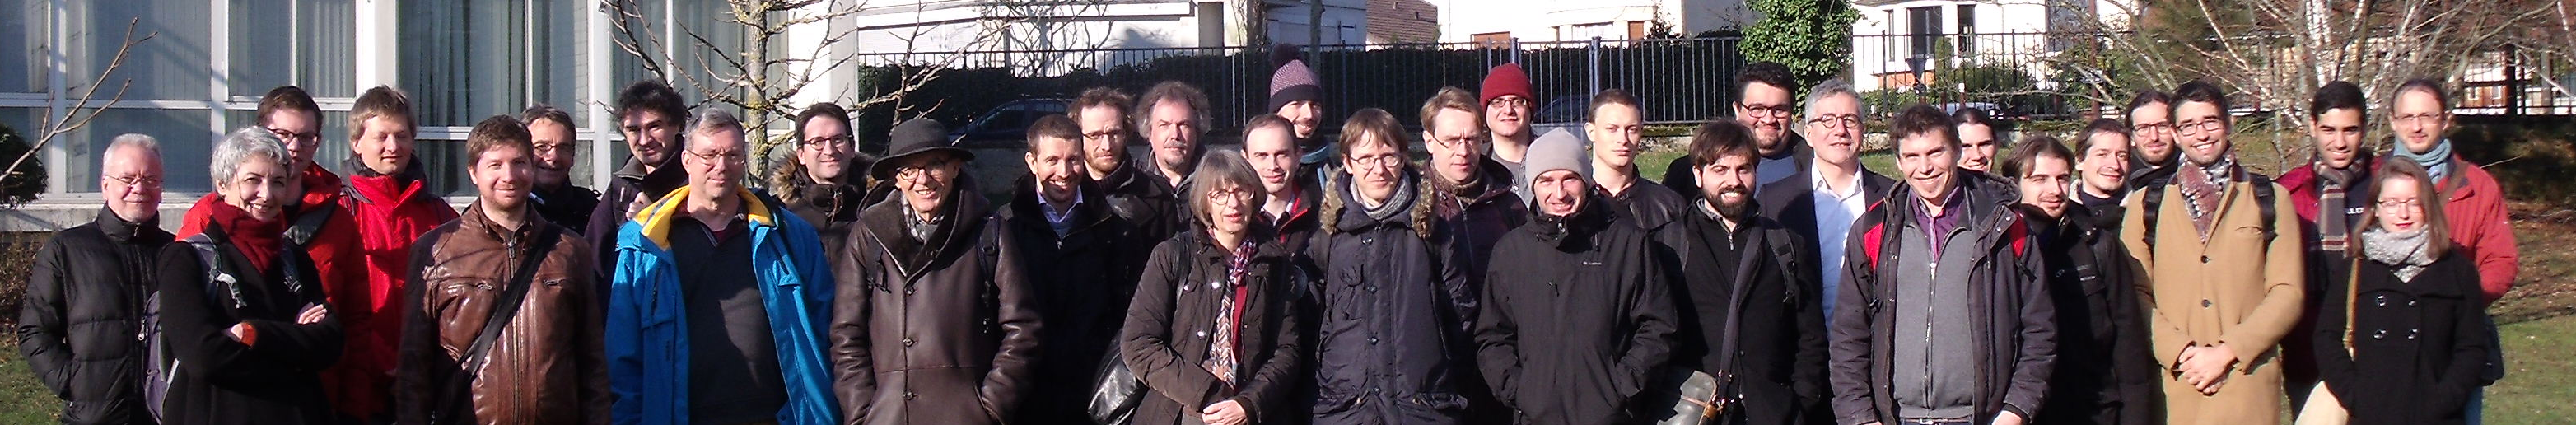
\includegraphics[height=2cm]{photo.png}
\end{center}
During this meeting, the idea of making this proof of concept a
European infrastructure emerged.  Since then, colleagues from Belgium,
Germany, Romania, Serbia, Sweden, and the United Kingdom, from
academia and industry, have expressed their interest in participating
in this effort.  These researchers and engineers are ready to
contribute to develop this encyclopedia, aiming at sharing proofs,
under a creative commons licence, making them searchable, accessible,
interoperable, and reusable.
\end{shaded}

%%%%%%%%%%%%%%%%%%%%%%%%%%%%%%%%%%%%%%%%%%%%%%%%%%%%%%%%%%%%%%%%%%%%%%%%%%%%%%
\begin{shaded}
\vspace*{-0.5cm}
\begin{center}
{\bf \Large How do proofs contribute to safety and security of software?}
\end{center}

Imagine the following casino game. At the beginning, a player is given
eleven euros. At each round, she throws a six-sided dice. If the
results is a six, then the game ends.  If it is a five, a four, a
three, or a two, she is given twice the amount of money she already
has. If it is a one she loses two euros, if she has at least two.
When the game ends, the player wins the money she got, except if she
has zero, in which case she loses one million euros.

This game can be modeled by the following programme:
\begin{center}
    \begin{minipage}{10cm}
\begin{verbatim}
n = 11
stay = True;
while stay:
    roll = random.randint(1,6)
    if roll == 6:
        stay = False
    else:
        if roll >= 2:
            n = n + 2 * n
        else:
            if (n >= 2):
                n = n - 2
print(n)
\end{verbatim}
    \end{minipage}
\end{center}

To be on the safe side, the player wants to be sure, before starting
playing, that she will never finish with zero.  And indeed, at all times
the content of the variable {\tt n} is an odd number,
thus it cannot be zero. {\bf This property ``nothing bad happens'' is
called the ``safety'' of this program.} This property is a
consequence of two simple theorems of arithmetic:
$$\forall x~(\mbox{\it odd}(x) \Rightarrow \mbox{\it odd}(x + 2 * x))$$
$$\forall x~(\mbox{\it odd}(x) \Rightarrow \mbox{\it odd}(x - 2))$$
meaning that, for all $x$, if $x$ is an odd number, then $x+2*x$ and $x-2$ are odd numbers too.
Hence, proving the safety of this programme amounts to prove these two
theorems.

Let's now consider the case where there is a tiny bug in the
program. For instance the {\tt 2} has been replaced by a {\tt 3} in
the instruction {\tt n = n + 2 * n}. The programme is then unsafe as
shown by the sequence $11, 9, 7, 5, 3, 1, 4, 2, 0$. Yet, testing this
program will, most likely, not reveal this bug, since it only
manifests very rarely.  In contrast, attempting to prove the
correctness of this program will reveal the bug as it is impossible to
prove the proposition
$$\forall x~(\mbox{\it odd}(x) \Rightarrow \mbox{\it odd}(x + 3 * x))$$
\end{shaded}

%%%%%%%%%%%%%%%%%%%%%%%%%%%%%%%%%%%%%%%%%%%%%%%%%%%%%%%%%%%%%%%%%%%%%%%%%%%%%%
%\begin{shaded}
%\vspace*{-0.5cm}
%\begin{center} {\bf \Large When mathematics are needed to verify the
%    correctness of a programme}
%\end{center}
%
%Prime numbers are used in a wide variety of applications:
%pseudo-random number generation, cryptographic algorithms, etc.  Thus,
%verifying the correctness of complex primality testing algorithms is
%critical.
%
%To do so, we need first to define primality, for instance
%
%$$prime(p) := 1<p \wedge (\forall n, (1<n\wedge n<p) \Rightarrow \neg(n\mid p))$$
%
%where $\wedge$ is the conjunction, $\Rightarrow$ is the implication,
%$\neg$ is the negation, and $n\mid p$ means that $n$ divides $p$.
%
%To lower the cost of primality testing, we use tests that are more
%efficient than the naive use of the definition.  For instance, a very
%simple improvement is to test the divisibility of the considered
%number, not by each of the smaller natural numbers, but only up to its
%square root.  Indeed, if a natural number $p$ can be factored into the
%product of two smaller natural numbers $m$ and $n$, one of them has to
%be smaller than or equal to the square root of $p$.  Therefore, one
%could give the following more complex, but more efficient, definition:
%
%$$prime'(p) := 1<p \wedge (\forall n, (1<n \wedge n*n\leq p) \Rightarrow \neg(n\mid p))$$
%
%To ensure that these definitions are equivalent one needs to prove
%the following statement:
%
%$$\forall p, prime'(p) \Leftrightarrow prime(p)$$
%
%It would have been easy to introduce a small bug
%in the new definition.  For example, one could have written
%$n*n < p$, instead of $n*n \leq p$.
%This would have resulted in accepting squares of primes as primes.
%
%Yet, attempting to prove the equivalence of these two definitions would
%have revealed the bug, as they cannot be proven to be equivalent.
%\end{shaded}

%%%%%%%%%%%%%%%%%%%%%%%%%%%%%%%%%%%%%%%%%%%%%%%%%%%%%%%%%%%%%%%%%%%%%%%%%%%%%%
\begin{shaded}
  \vspace*{-0.5cm}
  \begin{center}
    {\bf \Large What is a formal proof? What is a proof system?}
    \end{center}

Since Antiquity, we have known that
proofs, both purely mathematical ones, as in Euclid's elements or the
recent proof of the Kepler's conjecture by Thomas Hales, and proofs used
to establish the safety and security of software, can be built with a
limited number of rules, for example
\begin{itemize}
\item From $A\Rightarrow B$ (``$A$ implies $B$'') and $A$, deduce $B$.
\item From $A$, deduce $A\vee B$ (``$A$ or $B$'').
\item etc.
\end{itemize}
Yet for most of mathematical history, proofs have been written in
a pidgin of natural language and mathematical formulas. When proofs are
very long (as it is often the case for the proofs used in safety and security,
but also for some proofs in pure mathematics), mistakes are
very difficult to detect. For instance, dozens of wrong proofs of
the parallel postulate have been given through history, sometimes by the
best of mathematicians such as Ptolémée, Proclus, al-Haytam, Tacket,
Clairaut, Legendre, etc.

In the 1960s, Robin Milner and Nicolaas De Bruijn noticed that the
correctness of a mathematical proof could be checked by a
computer. This led to the development of the two first proof systems
in history: Milner's LCF and De Bruijn's Automath.

For instance, from the axioms
$$\forall x~(\mbox{\em philosopher}(x) \Rightarrow \mbox{\em human}(x))$$
$$\forall x~(\mbox{\em human}(x) \Rightarrow \mbox{\em mortal}(x))$$
we can deduce
$$\forall x~(\mbox{\em philosopher}(x) \Rightarrow \mbox{\em mortal}(x))$$
In the language implemented in Automath, this proof is written
$$\lambda x \lambda h~(g~x~(f~x~h))$$
\end{shaded}

%%%%%%%%%%%%%%%%%%%%%%%%%%%%%%%%%%%%%%%%%%%%%%%%%%%%%%%%%%%%%%%%%%%%%%%%%%%%%%
\begin{shaded}
\vspace*{-0.5cm}
  \begin{center}
{\bf \Large What is a theory?}
\end{center}

Deduction rules such as ``From $A \Rightarrow B$ and $A$, conclude
$B$'' are universal, but building proofs requires more rules, that are
often specific to a domain of knowledge and are called
``axioms''. Examples are the axioms of geometry, the axioms of
arithmetic, etc. These axioms constitute a theory.

At the beginning of the 20$^{\mbox{\footnotesize th}}$ century, an
axiomatic theory, {\em set theory}, has been proposed to express all
mathematical proofs. In the first half of the 20$^{\mbox{\footnotesize
    th}}$ century a few variants of set theory have been proposed, as
well as a few alternatives (such as \emph{Simple Type Theory}).  But
because these theories had not been designed for being implemented on
a computer, each proof system such as Coq, Isabelle/HOL, Mizar,
Atelier B, etc. implements its own theory.  {\bf Thus the rise of
computer-checked formal proofs has led to a multiplication of
alternative theories for mathematics.

This is the major obstacle to interoperability between proof systems.}
\end{shaded}

%%% Local Variables:
%%%   mode: latex
%%%   mode: flyspell
%%%   ispell-local-dictionary: "english"
%%% End:


\section{Objectives}

\begin{todo}{}\color{red}
  Describe the overall and specific objectives for the project1, which should be clear, measurable, realistic and achievable within the duration of the project. Objectives should be consistent with the expected exploitation and impact of the project (see section 2).
\end{todo}

\begin{figure}
\begin{framed}
  \begin{itemize}
\item[LIL 1:]
The theory implemented in the system has been defined in
the lambda-Pi-calculus modulo theory and in Dedukti.

\item[LIL 2:]
The system has been instrumented so some of its proofs can be exported
and checked in Dedukti.

\item[LIL 3:]
A significant part of the library of the system has been exported and checked in
Dedukti.

\item[LIL 4:]
A tool has been defined to analyze the Dedukti proofs for the system,
detect those that can be expressed in a theory weaker than that of the
system, and translate those proofs into a weaker logic.

\item[LIL 5:]
Certain proofs of the system have been made available in Logipedia.

\item[LIL 6:]
All proofs of the system have been exported, translated,
and made available in Logipedia.
\end{itemize}
\caption{The Logipedia integration levels (LIL)\label{lil}}
\end{framed}
\end{figure}

To foster the interoperability of proof systems and the sustainability
and the cross-verification of formal proofs, we propose to collect
them in an online encyclopedia, called {\sf Logipedia}.  For each
proof, {\sf Logipedia} will indicate in which systems it can be used
and, when this is the case, it will provide a version of this proof in
the theory of these systems.

Such a project will not only foster the use of formal proofs in
research in mathematics and computer science, but also in industry, by
allowing cross-verification, sustainability, and interoperability of
formal proofs, and in education, freeing the teaching of formal proof
technology from being bound to one system.

Such a project can only have a worldwide ambition. However, as a
majority of proof systems are developed in Europe, there is a unique
opportunity for Europe to take the lead on such a project and prepare
the grounds for the economic spinoffs from the project benefiting
European industry. That is why the consortium gathers most of the
European actors active on formal proof systems, while also developing
links with non-European partners.

Building this encyclopedia is {\em per se} a networking activity
between the partners, from academia and industry, involved in the
project.  Currently, we know how to express the theories of {\sf HOL
  Light} \cite{Assaf12}, {\sf Matita} \cite{Assaf15}, {\sf Coq} and
{\sf FoCaliZe} \cite{Cauderlier16} in {\sf Dedukti} and recheck proofs
developed in these systems.  We aim at including, in twenty years, all
formal proofs developed at that time.
In the next four years, we plan to address the theories of {\sf
  Abella}, {\sf Agda}, {\sf Atelier B}, {\sf HOL4}, {\sf Isabelle},
{\sf Minlog}, {\sf Mizar}, {\sf SMT-Lib}, \tlaplus, {\sf Why3}, {\sf
  LFSC}, {\sf PVS}, and {\sf TSTP}.  Other systems, such as {\sf
  ACL2}, {\sf IMPS}, {\sf Lean}, {\sf Nuprl}, and {\sf Rodin}, are
kept for later, except if some other partners join the project (Figure
\ref{systems}). This effort will require, and contribute, to build a
network of research teams, much stronger than what we currently have.

Beyond our main focus on interactive systems, we also plan to
integrate some proofs coming from automated theorem provers, SMT
solvers, and model checkers, when these proofs have a manageable
size. We already have experience with Archsat \cite{Bury19}, iProver
\cite{Burel10}, and Zenon \cite{CauderlierHalmagrand15}. We plan to go
further in this direction, in cooperation with our colleagues working
on LFSC \cite{Stump09}. Thus beyond the teams focused on formal proofs, we
will extend this network to teams of neighbour communities, such as
the automated theorem proving community and the SAT/SMT community.

To measure the level of integration of an existing proof system and
associated proof library in {\sf Logipedia}, we introduce a metric:
{\em the {\sf Logipedia} integration levels} (Figure \ref{lil}) that
counts six levels.  Among the 17 systems we shall focus on we plan to
increase the {\sf Logipedia} integration levels of 10 of them to level
5 or 6.

The various systems addressed in the project are currently at those levels:

\begin{tabular}{ll}
Matita:& level 5\\
FoCaliZe:& level 3\\
HOL Light:& level 5\\
Coq:& level 2\\
Agda:& level 2\\
Atelier B:& level 2\\
Isabelle:& level 2\\
HOL4:& level 1\\
TSTP:& level 1\\
Minlog:& level 0\\
PVS:& level 0\\
Abella:& level 0\\
Mizar:& level 0\\
TLA+:& level 0\\
SMT-Lib:& level 0\\
Why3:& level 0\\
LFSC:& level 0\\

\end{tabular}

and we plan to increase these levels to 

\begin{tabular}{ll}
Matita:& from level 5 to level 6\\
HOL Light:& from level 3 to level 5\\
FoCaliZe:& from level 3 to level 5\\
Coq:& from level 2 to level 5\\
Agda:& from level 2 to level 3\\
Atelier B:& from level 2 to level 5\\
Isabelle:& from level 2 to level 5\\
HOL4:& from level 1 to level 5\\
TSTP:& from level 1 to level ???\\
Minlog:& from level 0 to level 3\\
PVS:& from level 0 to level 2\\
Abella:& from level 0 to level 2\\
Mizar:& from level 0 to level 3\\
TLA+:& from level 0 to level 2\\
SMT-Lib:& from level 0 to level ???\\
Why3:& from level 0 to level ???\\
LFSC:& from level 0 to level ???\\

\end{tabular}

This encyclopedia will be freely accessible through a web browser,
from any country in Europe and beyond. But an important effort will be
made to make this encyclopedia accessible to a large community of
specialists and non-specialists, but structuring the contents on
libraries, books, chapters, etc. Some of the libraries we start with
already have a structure (modules, qualified names, etc.) that it is
important to preserve.

We shall also develop ergonomic interfaces, search engines, etc. 


Finally, this project will trigger joint research activities between
its users and between its developers.  First, there are several
theories for which we do not have yet reached level 1, and for which
we need to understand how to express then in {\sf Dedukti}. Which is
an obvious joint research activity. Then, we need to define algorithms
to eliminate some axioms from proofs. Many such algorithms already
exist to eliminate the excluded middle, the axiom of choice, or the universes
from a given proof. We need to develop new ones, more specific to the theories
we address in this project.

In addition, each library contains definitions of natural numbers,
real numbers, etc. and, most importantly, logical connectors, that
must be aligned, that is structural results proved for one definition
of real numbers must be transported to any definition of an isomorphic
structure.

All these objectives contribute to building a new formal proof
community, focused on the values of knowledge exchange and
sustainability.

%%% Local Variables:
%%%   mode: latex
%%%   mode: flyspell
%%%   ispell-local-dictionary: "english"
%%% End:



\section{Relation to the work program}

\begin{todo}{}\color{red}
  Indicate the work programme topic to which your proposal relates, and explain how your proposal addresses the specific challenge and scope of that topic, as set out in the work programme.
\end{todo}

\begin{longtable}{|p{0.2\textwidth}|p{0.75\textwidth}|}
\hline
{\bf Research \newline e-infrastructures for formal proofs}
&
Proof systems and automated theorem provers are research
infrastructures. Each proof system comes with its own library, and
these libraries are also part of the research infrastructure.  Currently
these infrastructures are small, distributed and disconnected.\\
&
\hspace{0.4cm}
Logipedia aims at building a large, worldwide infrastructure from the
small ones by integrating them.  The integration effort is substantial
because the proofs in the various libraries are expressed in different
theories, and because key definitions are formalized in a different
way.  But this integration effort is doable and contributes to the
challenge of bringing to European researchers and engineers effective and
convenient access to the best research infrastructures, in order to
foster further advances in knowledge and technology.\\
&
\hspace{0.4cm}
This idea to structure a networking activity around the construction
and the use of an infrastructure is relatively new in computer science
and mathematics. Moreover Logipedia is not an infrastructure of
computers, like Grid'5000 is, but mostly an infrastructure made of
data and of algorithms manipulating these data.  As Logipedia is an
e-infratructure, its budget structure is different from a material
infrastructure. A small part of the resources is used for computers,
and a large part of the budget is used to develop networking
activities, trans-national, virtual and ergonomic access, and joint
research activities.\\
\hline
{\bf A starting commu-}
&
This project has never been supported under FP7 or Horizon 2020 calls.\\
{\bf nity} &
\hspace{0.4cm} It mobilizes twenty nine research groups (twenty one in
academia and eight in industry), which is
almost all the groups working on formal proof technology in Europe.
The success of the project requires such a large network.  Indeed,
just like, according to Metcalfe's law, the effect of a network is
proportional to the square of the number of connected users, we can
postulate that the effect of an infrastructure, like Logipedia, is
proportional to the product of the number of proofs it contains and
the number of its potential users, each of them being proportional to
the number of theories it supports. So, such a project needs a
critical mass to succeed. This is also why we have developed a corona
surrounding the project, constituted of four clubs of users: 
a club of industrial users, a club of academic users, a club of users in 
education and a club of users in publishing.
These clubs
already have some members, but they will develop during the four years
of the project, preparing the long term future of the infrastructure.
The members of the club of industrial users have written letters 
explaining their interest in the project, that are in the appendix of this
document. {\color{red} Do not forget to include the letters.}
\\
&
\hspace{0.4cm}
These groups are located in eleven European countries.  Some of these
countries have a large number of participants, some others fewer,
reflecting the diversity of maturity of the research on formal methods
in Europe. This project will contribute to develop the formal proof
culture in the European countries where it is still inceptive.\\
&
\hspace{0.4cm}
We should also point out the originality of this project within the
European strategy of Research infrastructure.\\
&\\
&
$\blacktriangleright$ A novelty of this project is that is
investigates how infrastructures can be used in mathematics and in
computer science.\\
&\\
&
$\blacktriangleright$ It investigates how immaterial infrastructure
can be used to structure a research community, just like material ones
do.\\
&\\
&
$\blacktriangleright$ It is focused on mathematical {\em a priori}
knowledge, while most infrastructures are focused on {\em a
  posteriori} knowledge, issued from measures, observations,
experiments, and field surveys.\\
&\\
&
$\blacktriangleright$ It also investigates how a common infrastructure
articulates the relation between research and industry.
\\
\hline
{\bf Compliance policy with EU regulations}
&
A data management plan will be provided according to Inria’s
compliance policy with EU regulations. We also engage ourselves to
make the evolution of the Logipedia e-infrastructure compliant
with the European charter for access to research infrastructures.\\

\hline
{\bf Networking activities, trans-national access, joint re-}
&
Three work packages described below are dedicated to networking activities
to collect the data that constitute the infrastructure: the formal proofs
that constitute Logipedia.
\\
{\bf search activities}
&
\hspace{0.4cm}
Logipedia will be publicly and freely accessible online through any
web browser and trough a package management tool, so trans-national
and virtual access are provided directly. Its administration will be
decentralized in various places in Europe with two mirror sites in
Saclay and in München. But we go beyond trans-national and virtual
access.  Two work packages described below are dedicated to improving
the quality of the access to the encyclopedia.\\
&
\hspace{0.4cm}
Finally, this project fosters new joint research activities. First,
between the members of the consortium. Then, between the members of
the consortium and other academic partners, in particular those
developing automated theorem proving systems. Next, between the
consortium and the industrial users of proof systems. Finally, between
the industrial users themselves, as using proofs developed by others
will foster joint developments. Two more work packages are dedicated
to these research activities.  Such joint research activities
currently exist in Europe to some extent.  Such a joint project is a
unique opportunity to strengthen the existing ones and create new
ones.
\\
\hline
{\bf Towards standardization}
&
This project will be a stepping stone for a possible standardization
of proof languages.
\\
&
\hspace{0.4cm}
Unlike other communities in computer science, the formal proof
community is somewhat skeptical with respect to standardization. And
indeed, it would not make sense to standardize a theory for proof
systems, just like it would make no sense to propose Euclidean
geometry as a standard all geometers should use.  Instead, such a
cooperative effort can lead to the standardization of a logical
framework, that is a language to express theories and proofs in any of
these theories. Proceeding slowly and in a cooperative thus may change
the attitude towards standardization in the formal proof community and
make a standardization process more widely accepted.
\\
\hline
{\bf Inter-disciplinarity}
&
This project includes mathematicians, logicians, and computer
scientists and therefore is clearly inter-disciplinary.\\
&
\hspace{0.4cm}
Yet, Logipedia is inter-disciplinary in an even more fundamental
way. Proving properties of a piece of software driving a car or
piloting an aircraft require to formalize part of the physical world
in which this piece of software evolves. In the same way proving
properties of simulation software, requires to formalize some
properties of the simulated object.  Thus, just like mathematics and
software are involved in any part of modern science, formal proof will
eventually spread, over time, in all areas of science.\\
&
\hspace{0.4cm}
One major obstacle to the formalization of, for example, simulations
is that they typically depend on large bodies of knowledge in
mathematics and physics.  Different proof systems may be better
suited for different applications, thus there is a natural tendency
for a diversity of proof formats, just like there is a natural
tendency for diversity in the use of programming languages.  Yet, when
it comes to formalizing a particular physical simulation, one needs to
have all the necessary knowledge accessible from a single infrastructure.\\
&
\hspace{0.4cm}
Formal proofs will eventually become pervasive, and
different disciplines may be tempted to use different systems.
Because inter-disciplinarity is required to formalize physical world
simulations, a unifying language such as Logipedia for exchanging
formal proofs between theorem provers is a must-have.\\
\hline
\end{longtable}


%%% Local Variables:
%%%   mode: latex
%%%   mode: flyspell
%%%   ispell-local-dictionary: "english"
%%% End:


\section{Concept and methodology}

{\bf \Large (a) Concept}

\begin{todo}{Concept}\color{red}
Describe and explain the overall concept underpinning the project. Describe the main ideas, models or assumptions involved. Identify any inter-disciplinary considerations and, where relevant, use of stakeholder knowledge. Where relevant, include measures taken for public/societal engagement on issues related to the project;
  
Describe how the participating Research Infrastructures will be integrated to provide, at European and, where relevant, global level, an overarching Research Infrastructure service, contributing to structuring the European Research Area, and, where relevant, global cooperation on Research Infrastructures. Describe also how this ensemble will ensure complementarity and coherence with the existing European Research Infrastructures landscape, including ESFRI infrastructures and existing integrating activities for advanced communities;

Describe any national or international research and innovation activities which will be linked with the project, especially where the outputs from these will feed into the project;
\end{todo}

%%%%%%%%%%%%%%%%%%%%%%%%%%%%%%%%%%%%%%%%%%%%%%%%%%%%%%%%%%%%%%%%%%%%%%%%%%
\cmsection{Logical Frameworks}

The multiplication of systems and theories in which formal proofs are
developed jeopardizes the universality of logical truth. But it is not
the first time in history this has happened.  For instance, in the
19$^{\mbox{\footnotesize th}}$ century, the universality of logical
truth had been challenged in a similar way, by the non-Euclidean
geometries, as some statements could be true in one geometry, but
false in others.  At the beginning of the 20$^{\mbox{\footnotesize
    th}}$ century, a solution to this problem was found.  The
definition of the various geometries in predicate logic
\cite{HilbertAckermann} allowed mathematicians to understand which
axiom was used in which proof, restoring the universality of the truth
of judgements of the form ``the proposition $B$ is true under the
axioms $A_1, ..., A_n$''.

Predicate logic is not a theory {\em per se}, but it is a framework in
which one can express theories, as sets of axioms: a ``logical
framework''. As we shall see, expressing the various theories
implemented in Coq, Matita, Isabelle/HOL, PVS, etc.\ in a common
logical framework will permit, in a similar way, to analyze which
``axiom'' is used in which proof, and hence, in which theories this
proof is correct, and in which systems it can be used.

In 1928, predicate logic was a huge success, since three important
theories used at that time (geometry, arithmetic, and set theory)
could be expressed in it. But it also has limitations, which explains
that another of the major theories used at that time (Russell's type
theory, from {\em The Principia Mathematica}) has not been expressed
in it. Since then, several other theories, such as Church's Type
Theory \cite{Church40}, Martin-L\"of's Type Theory
\cite{Martin-Lof84}, and the Calculus of Constructions
\cite{CoquandHuet88}, have also been defined as autonomous theories,
and not in predicate logic.  These theories are those implemented in
most of the current proof systems.

This failure has led, in the field of proof systems, to the
abandonment of predicate logic, and even of the concept of logical
framework: the theories implemented in Coq, Matita, etc., are often
defined as autonomous systems, and not in a logical framework.

However, a different line of research has attempted to understand the
limitations of predicate logic and to propose more powerful logical
frameworks.  The most prominent limitations of predicate logic are the
lack of function symbols binding variables, the lack of a syntax for
proof terms, the lack of a notion of computation, the lack of a notion
of proof reduction for axiomatic theories, and the impossibility to
express constructive proofs. These limitations have led to the
development of other logical frameworks such as $\lambda$-Prolog
\cite{NadathurMiller88, MillerNadathur12}, Isabelle \cite{Paulson90},
the $\lambda \Pi$-calculus (also called the ``Edinburgh logical
framework'') \cite{HarperHonsellPlotkin91}, Deduction Modulo Theory
\cite{DowekHardinKirchner03, DowekWerner03}, Pure Type Systems
\cite{Berardi88,Terlouw89}, and ecumenical logics
\cite{Prawitz15,Dowek15,PereiraRodriguez17}.

All these logical frameworks have been unified in the $\lambda
\Pi$-calculus modulo theory \cite{CousineauDowek07}, implemented in
the system Dedukti \cite{Assaf16} on which Logipedia is
based. Geometry, arithmetic and set theory, but also Russell's type
theory, Church's type theory, Martin-L\"of's type theory, and the
Calculus of constructions can be expressed in this framework.

For instance, although the details are not important, Church's type
theory can be expressed in Dedukti, with 11 ``axioms'': 8 declarations
and 3 rewrite rules.

\begin{framed}
\vspace{-0.5cm}
\begin{center}
{\bf \Large Church's type theory expressed in Dedukti}
\end{center}

$\begin{array}{rcl}
type&:&Type\\
\eta&:&type \rightarrow Type\\
o&:&type\\
\mbox{\it nat}&:&type\\
\mbox{\it arrow}&:&type \rightarrow type \rightarrow type\\
\varepsilon&:&(\eta~o) \rightarrow Type\\
\Rightarrow&:&(\eta~o) \rightarrow (\eta~o) \rightarrow (\eta~o)\\
\forall&:&\Pi a:type~(((\eta~a) \rightarrow (\eta~o)) \rightarrow (\eta~o))\\
\\
(\eta~(\mbox{\it arrow}~x~y)) &\longrightarrow& (\eta~x) \rightarrow (\eta~y)\\
(\varepsilon~(\Rightarrow~x~y)) &\longrightarrow& (\varepsilon~x) \rightarrow (\
\varepsilon~y)\\
(\varepsilon~(\forall~x~y)) &\longrightarrow& \Pi z:(\eta~x)~(\varepsilon~(y~z))
\end{array}$
\end{framed}

So the theories implemented in various systems can all be expressed in
Dedukti and the proofs developed in these systems can be translated to
Dedukti. Just like in the case of non Euclidean geometry, this allows
the symbols and rewrite rules used in each proof to be analysed
\cite{Thire18,Dowek17} (a domain traditionally called ``reverse
mathematics'' \cite{Friedman76,Simpson09}) and to deduce in which
systems each proof can be used.  This analysis is the basis of the
interoperability between proof systems.

So, to make a formal proof, developed in some system $X$, accessible
to the users of other systems, the first step is to express the theory
$D[X]$, implemented in the system $X$, in the logical framework
Dedukti.  Then, we must instrument the system $X$ so that the proof
can be exported from it, as a piece of data, expressed as a proof in
$D[X]$ and included in Logipedia. Next, we need to analyze this proof
in order to determine which symbols, axioms and rewrite rules of
$D[X]$ it actually uses and, thus, in which alternative theories it
can be expressed.  Finally, we must align its concepts with the
definitions already present in Logipedia and decide where it fits in
the general structure of the encyclopedia.

%%%%%%%%%%%%%%%%%%%%%%%%%%%%%%%%%%%%%%%%%%%%%%%%%%%%%%%%%%%%%%%%%%%%%%%%%%
\cmsection{Integration of proof systems}

Consider a system $X$ at LIL 1, so the basic theory $D[X]$ has already
been expressed in Dedukti. The next step is to implement a method to
automatically translate proofs from system $X$ to its expression in
Dedukti, and make these proofs available in Logipedia so they can be
exported to other systems. This step is called the
``instrumentation'' of system $X$.

The systems we consider fall into three broad classes: the systems
based on dependent type theory, the systems based on simple type
theory, and those based on set theory and predicate logic.

\paragraph*{Systems based on dependent type theory (Agda, Coq, and Matita).}

Coq is an interactive theorem prover developed at Inria since 1984.
It is based on the Calculus of constructions and was used to formally
verify the correctness of both industrially relevant software such as
the CompCert C compiler and complex mathematical proofs such as those
of the Four Color theorem and the Feit-Thompson theorem. In 2013 Coq
received the ACM System Award.

Matita is an interactive theorem prover developed at the University of
Bologna and used for teaching logic courses and to verify software and
mathematical proofs, with special attention to predicative
foundations. The first generation of the system (up to version 0.5.9)
was born as a by-product of the MoWGLI FET-Open Project, it was
compatible with the logic of Coq and it could re-use its libraries. It
was an important test-bench for the integration of Mathematical
Knowledge Management techniques with Interactive Theorem Proving,
featuring for example a library of theorems distributed over multiple
servers, innovative indexing and search techniques and automatic
translation of proofs between declarative and procedural styles. The
second generation of the system (up to the current version 0.99.3) was
a re-implementation from scratch that departed from the logic of Coq
and that experimented with the most concise ways to implement an
efficient theorem prover. Several ideas later migrated into Coq. The
currently available largest library is the formal certification of a
complexity-preserving and cost-model-inducing compiler from C to
MCS-51 machine code, developed in the FET project CerCo (Certified
Complexity).

Agda is a dependently typed programming language and interactive proof
assistant developed at Chalmers University of Technology as well as
other places in Europe. The theory of Agda is similar to Coq and
Matita, but it is more focused on interactive development and direct
manipulation of proof terms (in contrast to using a tactic language to
generate the proof terms). To support the construction of proof terms,
Agda provides powerful features such as dependent pattern and
co-pattern matching, $\eta$-equality for functions and record types,
first-class universe polymorphism, and definitional proof
irrelevance. In addition, Agda provides an experimental option for
extending the language with user-defined rewrite rules, which are very
similar to the rewrite rules provided by Dedukti.

\paragraph*{Systems based on simple type theory (HOL4, HOL Light, and Isabelle/HOL).}

HOL4 is home to a few medium to large scale specifications and
associated proof developments that have value outside of HOL4. These
specifications include the formal semantics of the CakeML language
(and its verified compiler) and an extensive specification of the ARM
instruction set architecture (ISA) as formalised by Anthony Fox at the
University of Cambridge.

HOL Light is an implementation of Simple Type Theory.

Isabelle/HOL is an implementation of Simple Type Theory in the
Isabelle logical framework \cite{paulson700}. It sits in
between type-theory proof systems (like Coq or Agda) and classic
LCF-style systems (like HOL Light or HOL4).

\paragraph*{Systems based on set theory and predicate logic (Atelier B,  Rodin).}

Atelier B and Rodin are platforms or tools to develop models written
using the B method, a version of set theory expressed in predicate
logic.  A model in these systems expresses a state machine constrained
by invariant properties. Verification of the correctness of the model requires
discharging a number of proof obligations produced by a weakest precondition
calculus. For example, spanning tree algorithms, distributed
algorithms, and access control policies have been formalized
respectively in the EventB and (classical) B methods.  The development process for
both versions of the B method is based on formal proof: proof obligations are
automatically generated and must be proven by automatic or interactive
provers. This can include external solvers such as SMT solvers.

\bigskip

Despite the differences between these three classes of proof systems,
there are multiple common points between them where solutions that work
for one system can also be applied to other systems. Working together
on implementing these tools will allow the researchers from these
different communities to come together and learn more about the
similarities and differences between these systems.

Defining a basic instrumentation of some of these systems is
straightforward, but building tools that also work well in practice
raises new research challenges:


\paragraph*{Improving encodings.}
Even when we have understood how to express the basic theory of these
systems, implementation often reveals some advanced features of these
systems that require further work.  Moreover even when we know how to
express all features of some system \emph{in theory}, depending on the
choice of expression, the instrumentation may be simpler or harder in
practice. For example:
\begin{itemize}

\item Many Agda libraries (as well as some Coq libraries) rely heavily
  on type-directed conversion rules such as $\eta$-equality for functions
  and record types, or definitional proof irrelevance. These rules
  have to be expressed by adding type information to the
  proof terms. This can in turn lead to a large blow-up in the size of
  those proof terms, and thus greatly increase the cost of
  typechecking. This blow-up has to be tamed by the choice of a
  clever expression of the theory.

\item Coq, Agda, and Matita all provide support for coinductive
  (infinite) structures, which can be expressed by rewrite rules in
  Dedukti, but this expression must be carefully chosen so that the
  proofchecker does not go into an infinite loop.

\item A few of the systems rely on AC rewriting (i.e.~rewriting modulo
  associativity and commutativity of certain operations), for example
  to express universe polymorphism in dependent type theories. While
  Dedukti has support for AC rewriting, the current implementation is
  very slow, which makes typechecking the proofs in Dedukti
  infeasible. Thus, expressing these theories efficiently requires improvements in
  Dedukti itself.
\end{itemize}

Finding better ways to express such features could have a great impact
on the quality and speed of the translation process.  We plan to
investigate two possible approaches to improve the expression of
common features of proof assistants in Dedukti. First, we will
investigate whether some information in the current expressions is
redundant and can thus be omitted. Second, if this is not possible, we
will investigate what minimal changes need to be made to Dedukti
itself in order to overcome these limitations.

\paragraph*{Reconstructing transient proof components.}
In all proof systems, there is some information that is created during
the process of checking a proof that is not stored in the final proof
term. In systems such as Coq, Agda, and Matita, this concerns for
example the types of each subexpression. In other systems such as
HOL4, Isabelle, and Atelier B, even more information about the proof
is discarded and only the high-level proof steps remain.  However, the
translation from the system to Dedukti might rely on this transient
information. Developing a method to reconstruct this transient
information is thus crucial.

In order to instrument systems with transient proof information, the
proof terms need to be complemented with this transient information by
either logging or re-synthesizing it on demand. Both approaches may be
used, depending on the the trade-off between computation time and space
for storage.

However, this approach is insufficient for systems that rely on
external provers such as Isabelle or Event B. In order to handle these
cases, we will instrument these external provers so they can produce
the missing parts of the proof terms.

\paragraph*{Producing more compact proofs.}
When translating a proof from some external system to Dedukti, we want
to produce proof terms that are as small as possible, so it is easy to
store them, recheck them, or export them to a different
system. However, there are at least two reasons why proof terms might
become large. First, a typical proof in an external system may be large
(because big parts of it are constructed automatically). Second,
translating a proof to Dedukti may increase the size of the proof, for
example by normalizing it or by adding type annotations.  This means
translating the proofs can take a very long time, and doing anything
with the translated proof will be difficult. This also has an obvious
impact on the exporting of large libraries to Dedukti, discussed
below.

To reduce the size of proof terms produced by the translation to
Dedukti, we plan to investigate how to avoid unnecessary
normalization or duplication of (parts of) proofs. We will also
investigate what parts of each proof can be safely omitted because
they can be inferred from the rest of the proof.

\bigskip

For each of the systems considered in this project, we can identify
some preliminary work, of varying maturity, on translating proofs to
Dedukti.  We plan to build upon the previous work done for the
following systems:
\begin{itemize}
\item The standard and arithmetic libraries of Matita have been the
  first libraries to be exported to Logipedia using Krajono, a fork of
  Matita. We plan to make this translation a part of the code of
  Matita itself so that it is maintained with the rest of the system.

\item The standard library of HOL Light and FoCaLiZe already have been
  translated to Dedukti.

\item CoqInE is a prototype tool that can translate Coq proofs to
  Dedukti. Recent work to include advanced features of Coq, such as
  universe polymorphism, has dramatically increased the coverage of
  this translation. We plan to make this translation a part of the
  code of Coq itself so that it is maintained with the rest of the
  system.

\item In the summer of 2019, Guillaume Genestier worked together with
  Jesper Cockx on the implementation of an experimental translator
  from Agda to Dedukti during a research visit at Chalmers University
  in Sweden. This translator is still work in progress, but it is
  already able to translate 142 modules of the Agda standard library
  (about 25\%) to a form that can be checked in Dedukti. This
  exploratory work uncovered several challenges and opportunities for
  further work (see research challenges above).

\item The inference kernel of Isabelle has already been instrumented
  to output proofs as $\lambda$-terms that can be understood by
  Dedukti. However, this has so far been only used for small examples
  \cite{Berghofer-Nipkow:2000:TPHOL}. The challenge is to make
  Isabelle proof terms work robustly for the basic libraries and
  reasonably big applications.  Preliminary work by Wenzel (2019) has
  demonstrated the feasibility for relatively small parts of
  Isabelle/HOL, but this requires scaling up.

\item HOL4 has support for exporting proofs to the OpenTheory proof
  exchange format, and there has been some work on importing
  OpenTheory proofs into Dedukti.

\item In the context of the BWare project, an expression of the set
  theory of the B method has been provided as a theory modulo, i.e.\ a
  rewrite system rather than a set of axioms. This expression is used
  by the automatic prover Zenon modulo which features a back-end to
  Dedukti. Thus, as a first step through instrumentation of Atelier B
  proof obligations coming from Atelier B can be proved by Zenon
  modulo producing Dedukti proofs, hence providing a better confidence
  in the proofs produced by the native proof tools of Atelier B
  \cite{Bware}.
\end{itemize}

The success of this integration project is measured by the LIL of the various
considered systems at the end of the project.

\cmsection{Automatic theorem provers, SAT/SMT solvers, model checkers, etc.}

We have previously discussed the instrumentation of \emph{interactive}
proof systems such as Coq, Isabelle/HOL, Agda, etc.,
where the users build formal proofs with the help of the
machine. Automatic theorem provers are another class of systems, where
the machine builds proofs without any human intervention. The proofs
built by these systems are often expressed in simpler theories than
those developed using proof systems, but they are not of a different
nature.  They cover various domains and various kinds of application,
{\em e.g.}  combinatorial
mathematics~\cite{DBLP:journals/ai/KonevL15,DBLP:conf/sat/HeuleKM16},
where they are expected to solve one large propositional problem, or
proof of
programs~\cite{DBLP:conf/esop/FilliatreP13,DBLP:journals/pacmpl/ProtzenkoZRRWBD17},
where they are given thousands of small problems in a combination of
quantified theories.

Including proofs built by such automatic systems in Logipedia,
whether they are called automatic theorem provers, SAT solvers, SMT
solvers, etc. is both a goal {\em per se}, and a tool to help to
integrate proofs developed in proof systems and make a coherent whole out
of Logipedia. A fruitful interaction between formal proofs requires
low-level glue which falls in the scope of automatic theorem provers.
For instance, they will be employed to fill the holes that appear when
considering provers with various granularity, to reduce the gaps
between proof systems, and to discharge proofs of concept alignment.

On the other hand, automatic theorem provers will also benefit from
Logipedia. Obviously, Logipedia will be an extensive library of formal
statements that can be used and combined by automatic theorem provers
in their proof search. This is not trivial though: automatic theorem
provers have to select the right lemmas for a proof, which becomes
more difficult the more lemmas there are. It can also be a source of benchmarks to
evaluate their expressivity and automation.  Lastly, Logipedia and
Dedukti will form a framework to make automatic theorem provers
cooperate with each other and with other tools, in a safe way.

\subsubsection*{From automatic theorem provers to Dedukti}

Similarly to interactive theorem provers, connecting automatic theorem
provers to the Logipedia infrastructure strongly relies on the ability
for automatic theorem provers to import statements from Dedukti and
export proofs in some theory in Dedukti.


\paragraph*{Instrumenting automatic theorem provers to produce proof traces.}
The first step for connecting automatic theorem provers to the
Logipedia infrastructure, and the library of proofs, is that automatic
theorem provers should actually output some kind of proof, without
enforcing strong requirement on the format or even the level of
granularity of those proofs.  SAT (satisfiability) solvers for
propositional logic do have a perfectly well specified format for
proof traces~\cite{TODO} and most SAT solvers are actually able to
produce proof traces in that format.  So, considering SAT solvers, the
current status is actually meeting the Logipedia needs on this aspect.

Considering other automated reasoners however, it is necessary to
significantly improve the picture.  Some SMT (Satisifiability Modulo
Theories) solvers do produce some kind of proof trace, but the format
is specific to the solver, and the proofs are sometimes difficult to
replay due to their (lack of) granularity.  Most mainstream theorem provers for
predicate logic output proofs in a standardized language~\cite{TODO},
but this language does not clearly specify the semantics of the proof
steps.  Model-checkers do not provide proof traces {\em per se}, although
such traces would be useful for various usages and notably
certification.

Our goals are to improve reasoning tools to demonstrate the
feasibility of producing sufficiently detailed proofs for connecting to
Logipedia, and to design a set of theoretical methods and practical
tools that can be used to further connect Logipedia to the other
existing automated reasoners of the same kind.  We will work on three
SMT solvers (Alt-ergo, CVC4, VeriT), two provers for predicate logic
(the E-prover, Zipperposition), and one model-checker (Cubicle).  We
will also consider more specific reasoning tools, with the aim to
demonstrate that this approach also applies to more specific
reasoners.  We envision to experiment with this approach on a reasoner
for Coherent Logic.  These reasoners are particularly useful for geometric
reasoning, and as such, they are quite complementary to the other
automatic reasoners considered.  They are also very suitable as as a
first experiment, since their proofs are fairly straightforward to
interpret.  They thus constitute a very interesting low hanging fruit.

It is not possible, and not even desirable, to require all tools to
directly talk in the language of Logipedia.  Indeed, proof trace
languages that are specific to one kind of reasoning tool are more
appropriate than Dedukti for instrumenting already large pieces of
software, enabling quick output, and allowing post-processing the
produced proof traces at the right level of abstraction.
Furthermore, provided that those proofs are detailed enough,
translation of traces to Dedukti will not be a difficult task, and
the work necessary to translate proof traces for a myriad of very
different reasoners will be implemented in a single tool (Ekstrakto,
see below) to take advantage of the fact that there is quite a lot of
sharing of reasoning techniques, and thus proof methods, among the
solvers.

\paragraph*{Translate automatic theorem provers traces into Dedukti.}
As pointed out above, it is easier to instrument provers to make them
output traces, instead of directly provide Dedukti proofs. The second
step to connect automatic theorem provers to the Logipedia
infrastructure is to reconstruct the proof traces in order to build
Dedukti proofs from them. The proposed process is the following: each
step of the trace is transformed into an independent sub-problem; each
of these sub-problems is given to a prover that can output Dedukti
proofs; proofs of the sub-problems are then combined to produce a
global proof of the original problem.  Since sub-problems correspond
to atomic steps of the proof trace, they are relatively simple, so
that we are confident that the prover producing Dedukti proofs will
not struggle to find a proof. This process is quite similar to what is
done by the hammer tools of interactive theorem provers (Sledgehammer
in Isabelle/HOL, HOLyHammer for HOL4, etc.) which reconstruct proofs
from traces produced by automated theorem provers.

This scheme has already been prototyped in a tool called
Ekstrakto. Ekstrakto takes a TSTP file, as can be produced by
e.g.\ the provers E and Zipperposition, and it uses Zenon Modulo and
ArchSAT to prove the sub-problems. Ekstrakto was designed to be
agnostic with respect to the prover producing the trace; in particular
it does not depend on the specific set of inference rules of the
prover. It was also designed to be agnostic w.r.t.\ the prover used to
prove the sub-problems; it is only required that the prover can output
a Dedukti proof in the correct expression of predicate logic.

Although work on Ekstrakto has already shown that approach is valuable,
it is a work in progress. In particular, the following issues will be
addressed in the project:

\begin{enumerate}
  % extension to other proof trace formats
\item Up to now, Ekstrakto can only understand traces in TSTP format as
  input. We plan to make it accept traces in other formats, notably traces
  from SMT solvers, as well as all formats that will appear when instrumenting
  other automatic theorem provers.

  % unprovable steps
\item Some steps in the proof traces are not provable: their
  conclusion is not a logical consequence of their premises. However,
  they preserve provability: the original problem has a proof if and
  only if the problem with the conclusion of the step also has a
  proof. This is the case for instance of the Skolemization step an
  automated theorem prover for predicate logic, of the introduction of
  new definitions, as well as the RAT property in traces produced by
  SAT solvers. The approach of Ekstrakto cannot be used here, because
  the sub-problem corresponding to the step cannot be proved. However,
  since provability is preserved, it should be possible to transform a
  proof using the conclusion of the step into a proof using its
  premises. Such a transformation depends on the nature of the step
  that has been used. We plan to include in Ekstrakto a way to handle
  Skolemization and definition introduction, which are the two step
  families that are missing to be able to manage all traces from the
  major theorem provers for predicate logic.

  % specialization for theories

\item Dedukti-producing provers used by Ekstrakto, namely Zenon Modulo
  and ArchSAT, are meant for pure predicate logic. However, we would
  like to deal with proof traces that use some specialized theory,
  e.g.\ arithmetic or bit-vectors, as could be output by SMT
  solvers. Although such theories could be presented as a set of
  axioms in predicate logic, it is almost certain that neither Zenon
  Modulo nor ArchSAT could be able to find non-trivial proofs using
  these axioms. Here, the idea would be to develop small provers
  dedicated to a particular theory that can output Dedukti
  proofs. Such provers would be called when a step in the trace relies
  on said theory. These provers need not be very optimized, since
  trace steps are relatively small; this should help producing Dedukti
  traces. A way to achieve this could be to extend Zenon Modulo:
  indeed, Zenon modulo can find proofs modulo arithmetic, but it is
  not able to produce a Dedukti proof yet.
\end{enumerate}

\subsubsection*{From Dedukti to automatic theorem provers}

%\label{concept:wp4:deduktitoatp}
In the other direction, Logipedia will constitute a source of
knowledge for automatic theorem provers. For this to be affordable,
this project will study the following challenges.

\paragraph*{Translate Dedukti statements into automatic theorem provers
  inputs.}
Automatic theorem provers are mostly based on (parts of) predicate
logic.  Logipedia theorems, which mostly come from interactive
provers, will be expressed in the Dedukti encodings of much more
expressive logics, such as dependent type theory or simple type
theory.  Theorem statements thus need to be expressed in a different way
to be manipulable by automatic theorem provers.

Encodings of expressive logics in predicate logic already exist,
and are used for instance in {\em hammers} for using automatic theorem
provers into interactive theorem
provers~\cite{DBLP:conf/lpar/PaulsonB10,DBLP:journals/jar/CzajkaK18}.
In these tools, the encodings are specific to one system to be
affordable. In Logipedia, we have to combine and take benefit from
statements coming from the encodings of different systems based on
different logics. The key challenge here are thus:
\begin{itemize}
\item to avoid the loss of meaning arising from a succession of
  encodings; and
  \item to encompass statements coming from different systems.
\end{itemize}

We plan to investigate a new approach where, instead of hammers, the
encoding is a succession of fine-grained encodings dedicated to one
aspect. These ``small'' encodings will offer the possibility to be
activated independently depending on the origin of the statement. In
addition, they have the other advantages of being modular, easily
extensible, and more reliable: each encoding is simple, and may output
proofs, {\em e.g.} using Ekstrakto. They will be performed modulo the
concept alignment.

It is common in the automatic theorem proving community to evaluate
the performance of a particular tool on sets of benchmarks. As a side
effect of our work on integrating automatic theorem provers, we will
be able to extract a new set of benchmarks from Logipedia to measure
the performance of automatic theorem provers on problems coming from
different logics, and from a combination of these logics. In our case,
it will not only allow to compare automatic theorem provers but also
to measure the success of this task by evaluating the quality of the
encodings, and comparing the impact of each of our ``small'' encodings
by activating or deactivating them individually.

\paragraph*{Logipedia as a source of knowledge for automatic theorem provers.}
The amount of knowledge available in the whole of Logipedia is
significantly larger than in any library of an individual proof assistant,
and as such selecting the knowledge relevant for a
particular goal might require more complex techniques than
before~\cite{Irving-deepmath}.  We will experiment with integrating techiques
from machine learning to the construction of formal proofs. This includes both techniques
for selection of relevant knowledge for a goal and for the selection
of most promising constructors in the direct proof term
construction~\cite{ZielenkiewiczSchubert2016}.

\subsubsection*{Large scale application: formal verification of C code}

The use of formal methods in the industry requires to have approaches
that apply to a wide variety of cases. For the verification of C code,
the Frama-C platform features numerous techniques. One of them relies
on automatic solvers: Frama-C-WP. Since automatic theorem provers are
built by making many choices, such as which heuristics or which
algorithms to use, they display blind spots where they are less
efficient to solve some cases. To overcome this limitation, it is
necessary to use a wide variety of solvers in a portfolio manner. For
instance, the Why3 tool features the ability to send problems to lots
of provers in a uniform way. However, with so many tools written by
different teams, the meaning of the same concept in the different
tools could be different. This can lead to errors in the overall
verification results. Moreover, in order to be applied more widely,
formal methods must handle more concepts such as floating point
numbers whose exact meaning is less clear that mathematical
integers. This leads to more chances for two tools to interpret the
same concept differently. Finally, industrial users sometimes need to
add a kind of reason or a simplification that is specific to their
particular concept, so that it is better handled by automatic
solvers. It is very easy to make an error in those simplifications.

In order to overcome these problems, we propose to improve the assurances in
the interaction between these different tools, and to speed up the addition of
new features for handling new cases by using proof objects:
\begin{itemize}
\item For the industrial users who need to define the concepts they want
  to verify in their C code, we will add the possibility to import
  concepts from Logipedia. The user gains time by not having to define
  these concepts themselves and by being able to use proofs for accompanying
  lemmas.

\item For writing the simplification rules for industrial use cases,
  we will instrument Frama-C-WP to generate
  Ekstrakto input in order to produce a proof of the correctness of
  these simplifications.

\item For transforming problems to fit the different provers
  in Why3, we will take inspiration from the fine-grained encodings
  (see above) to also generate an Ekstrakto proof.

\item In the end, we will gather the Dedukti or Ekstrakto proofs of the
  provers, the encodings, and the simplification rules, in order to
  assemble them in a coherent whole.
\end{itemize}

This part thus combines and validates most of the previous aspects of
automatic theorem proving, but also constitutes the
challenge to instrument a large-scale formal tool for transforming
and combining proofs extracted from automatic theorem provers.

\subsubsection*{Automatic theorem provers to increase Logipedia readiness}

Providing automation on the level of an encyclopedia of formal proofs
is both interesting and challenging. Indeed, making so many different formal
systems cooperate requires a lot of proof manipulation,
transformations, and gluing, which can only be reasonably done with
automation. On a higher level, being able to more efficiently write
proofs directly in Dedukti would also be of interest to the community in
itself. Thus a major challenge is to make this automation practicable and scalable.

\paragraph*{Automatic theorem provers for Dedukti.}
Automation has been a key to the success of proof assistants, since it
allows much more efficient formalization~\cite{Hales-Developments}.
Many different techniques to provide proof assistant automation have
been developed over the years: techniques based on rewriting,
tableaux~\cite{Paulson-blast}, or even the integration of efficient
superposition-based provers for predicate logic~\cite{hurd-metis} and
simple type theory~\cite{asperti-matita-paramodulation}. Most
recently, various machine learning techniques have been developed for
proof assistants allowing for more precise selection of relevant
knowledge~\cite{blanchette-h4qed-jfr} or even the prediction of useful
proof techniques~\cite{gauthier-tactictoe}.

The automation techniques offered by different proof assistants differ
significantly. For systems mostly based on classical predicate logic
it is often possible to provide sound and complete translations to the
existing efficient theorem provers for predicate logic by only
expressing the intricacies of their type
systems~\cite{kaliszyk-miz40}. This allows for straightforward native
proof reconstruction. On the other end of the spectrum, for
systems based on involved foundations, such
as the constructive type theory behind Coq and its variants,
providing even a slightly useful automation is a significant
challenge. Most efficient automation still relies on translations to
external tools, but the current translations from such logics to
the logic of SMT solvers~\cite{DBLP:conf/cpp/ArmandFGKTW11} or
predicate logic~\cite{DBLP:journals/jar/CzajkaK18} are incomplete
and often (partially) unsound. This means that to reconstruct such
proofs in the logic of the proof assistant separate intricate
components need to be developed.

As part of the project we will experiment with various kinds of proof
automation on the level of Dedukti and verify their applicability to
the different libraries imported as part of the Logipedia project.
Furthermore, we will experiment with machine learning techniques for
formal proofs. This includes both techniques for selection of relevant
knowledge for a goal and for the selection of most promising
constructors in the direct proof term
construction~\cite{ZielenkiewiczSchubert2016}. Finally we plan to look
at computational proof reconstruction, to complement the link to
automated theorem provers developed in the other parts.

\paragraph*{Automation for Logipedia.}
The aforementioned automation will be crucial to enable full proof
verification. Considering systems one at a time, a number of proof
exports are not complete, i.e.~the actual systems do not provide
all the proof step details and internal automation for Logipedia would be
necessary. More demandingly, automation will be used to fill the gaps
between systems. In particular, concept alignments need to be established
formally. More generally, proof obligations arising from translations,
encodings into Dedukti, reverse mathematics, \dots must be discharged
as automatically as possible.

As it has been the case for interactive theorem provers, automation
will also provide support for Logipedia developers and users. During
the project, many Dedukti developments shall be performed, in
particular to define theories in Dedukti. In the longer term, Dedukti
will also be used, {\em e.g.} for new proof transformations or to
align distant concepts, which will be affordable with automation.

The success of the integration of proofs coming from automated theorem
proving systems, SAT solvers, SMT solvers, and model checkers, can be
measured by the size of the proofs imported from these systems to Logipedia.

%%%%%%%%%%%%%%%%%%%%%%%%%%%%%%%%%%%%%%%%%%%%%%%%%%%%%%%%%%%%%%%%%%%%%%%%%%
\cmsection{Large libraries}

We have seen how to instrument proof systems and automated theorem
provers to produce proofs in Dedukti, and how to share these proofs in
Logipedia.

Very large proofs, requiring large libraries of auxiliary results,
have been developed in some proof systems. These large proofs and
libraries are interesting for our project in two respects. First, they
constitute an excellent benchmark for the methods developed
above. Secondly, they will serve as the source for the lion's share of
proofs in Logipedia for end-user applications.

The libraries we target are dedicated to particular application
areas. They provide a substantial coverage of one application area
and do so in a structured manner. Thus integrating it into a general encyclopedia
may require reworking the libraries for better access. Any library
is only as useful as its structure and documentation.

The libraries are curated for end-user application. That is, they are
structured according to application specific ontologies that support
browsing and search. This structuring leverages the infrastructure
and will be a stress test for the results of structuring discussed
below: is our metadata infrastructure capable of representing the
structure of large libraries?

The libraries we focus on have been selected according to the
following criteria:
\begin{itemize}
\item Relevance: the libraries should support core areas of mathematics
  and computer science.
\item Coverage: the libraries should have a wide coverage of an
  application area.
\item Maturity: the libraries should have been used in a significant
  application already.
\end{itemize}

As a result we selected the following libraries: the Archive of Formal
Proofs, Isabelle's revised Analysis and Probability library, GeoCoq,
Flyspeck and CakeML.  Other very interesting libraries such as
MathComp, Coq's revised Analysis library, CompCert, seL4, and selected
Mizar and PVS libraries are left for future work.

\paragraph*{Isabelle's Archive of Formal Proofs.}
Isabelle's Archive of Formal Proofs (AFP) \cite{isabelle-afp} is a
growing user-contributed online library for Isabelle. In Feb-2020, the
Archive of formal proofs consisted of more than 500 entries (articles of formalized
mathematics) by 340 authors, and required approx. 60h CPU time for
checking (using many gigabytes of memory).  The purpose of this task
is to scale up the Isabelle instrumentation for Dedukti further, to
cover major parts of this library. We do not intend to restructure or
document the library further beyond what is provided by the authors of
each article and by the hierarchical dependencies among the articles.

The key challenge is scaling. The ultimate aim is to export the main
substance of the Archive of formal proofs without promising full coverage: some entries
with prohibitive resource requirements will be omitted. Also note that
the Archive of formal proofs is continuously growing at a high rate and thus a moving
target.

\paragraph*{The Isabelle Analysis \& Probability Theory Library.}
The Isabelle Analysis \& Probability Theory Library consists of more
than 200.000 lines of definitions and proofs, corresponding to almost
4000 printed pages. It covers topology, homology, multivariate,
functional and complex analysis, measure and probability theory, and a
dedicated library for ordinary differential equations. It is fair to
say that it is the most advanced machine-checked library in the area
of analysis and probability theory. The Isabelle analysis and
probability theory library is in part based on the extensive library
of the HOL Light system but has generalized it from real numbers to
appropriate algebraic structures and includes areas absent from the
HOL Light library (in particular measure theory and ordinary
differential equations). It is currently used by 60 out of 500
articles in the Archive of Formal Proofs, a user-contributed library
of Isabelle/HOL proofs from all areas of computer science and
mathematics. Moreover, it is the only existing library in this area
where proofs are structured and readable. Due to its size and
generality and because analysis and probability theory are pervasive
in any application in the engineering and natural sciences and
economics, this library is a key exploitable result of the project: it
is a fundamental enabling resource for almost any formal verification
activity in these areas, for example autonomous driving and
mathematical finance. The purpose of this task is to structure,
document and develop this library for optimal accessibility, ease of
use and comprehensiveness. The aim is a curated library for
applications.  Therefore some material will need revising for ease of
use and some essential material will need to be added.

\emph{Accessibility:}
The library is a large collection of theories with a hierarchical dependency
relation. However, this structure has grown over time and does not always
reflect the abstract mathematical dependencies. In short, the structure needs
to be modularized. This requires a significant refactoring effort.
%
At the same time we need to add metadata to the source material to turn this
structured collection of theorems and proofs into a curated library at the
Dedukti level (see below). The Analysis \& Probability Theory library will be
used as a first test case of the infrastructure
for handling metadata that will also be developed in this project, in
particular the ability to describe ontologies for structuring in the large.
This will entail in particular annotating those statements in the library that
correspond to proper mathematical theorems as opposed to auxiliary lemmas
required only for the benefit of the theorem prover.
To increase accessibility we will also include links from the library into
Wikipedia and in particular in the other direction to raise the awareness
of Logipedia.

\emph{Development:}
Although the library support for integrals is extensive, it suffers
from the (necessary) coexistence of different kinds of
integrals. This complicates proofs about integrals in applications and needs
to be unified, which entails further refactoring. The rest of the
development adds further essential material:
\begin{enumerate}
  \item Fourier analysis because of its extreme importance both for pure mathematics and for
engineering and physics (especially the Fourier
transform). A formalization of basic properties of the Laplace transform is already available in the Archive of formal proofs.
\item Stability theory for differential equations and
dynamical systems, in particular Lyapunov functions, because of their
relevance for the verification of cyber-physical systems.
\item Stochastic differential equations to model a large range of
dynamical systems with stochastic components, from physics to financial markets.
\end{enumerate}

\paragraph*{The GeoCoq library.}
The GeoCoq library consists of more than 100.000 lines of definitions
and proofs in geometry. It is mostly based on synthetic approaches,
where the axiom system is based on some geometric objects and axioms
about them, but, following Descartes and Tarski, it proves that the
analytic approach can be derived, where a field $F$ is assumed
(usually $\mathbb{R}$) and the space is defined as $F^n$. Moreover, it
contains a model, based on the analytic approach, of one of the
synthetic approaches present in the library, namely Tarski's system of
geometry, thus establishing the connection between these two
approaches in the opposite direction.

The fact that the analytic approach can be derived from the synthetic
one is called the arithmetization and coordinatization of geometry and
it represents the culminating result of both Hilbert's {\em Grundlagen der
Geometrie} and Tarski's {\em Metamathematische Methoden in der
Geometrie}. As of now, there is no other formalization of this result
inside a proof assistant, making the GeoCoq library the most advanced
machine-checked library in the area of synthetic geometry. This
formalization enables to obtain automatic proofs based on geometric
axioms using algebraic automated deduction methods, some of which will
be covered by automated theorem proving.

The main axiom system in this library is the one of Tarski, but
Hilbert's axiom system and a version of Euclid's axioms sufficient to
prove the propositions in Book 1 of Euclid's Elements are also
defined. Thanks to the proof that Tarski's axioms (except continuity)
are equivalent to Hilbert's axioms (except continuity), the
arithmetization and coordinatization of geometry are available for
both systems. In the library, the focus is not only on axiom systems
but also on axioms themselves. Eleven continuity axioms are available
and are hierarchically organised. Finally, it contains a new
refinement of Pejas' classification of parallel postulates together
with proofs of the classification of 34 versions of the parallel
postulate.

\emph{Challenges:} A lot of preliminary work has been done on making the
GeoCoq library available in Logipedia.  One of the remaining obstacles is the use of
computational steps in Coq proofs. The issue is that proofs making use of
proof by reflection reach a level of complexity that currently makes
verification by Dedukti impractical, but these proofs are very
frequent in Coq.  One possible approach is to isolate these proofs by
reflection so that they are not perceived as simple conversion steps
in the type theory proofs, but marked as proofs to be treated by an
automatic tool. The coherent logic theorem prover should handle part
of these proofs. The other ones should be handled by specific provers
for geometry, as they correspond to proofs obtained by the Gr\"obner
basis method in GeoCoq.  Another challenge is that CoqInE, a tool
developed to translate Coq proofs into Dedukti type-checkable terms,
produces terms in an encoding of the Calculus of Inductive
Constructions into the $\lambda \Pi$-calculus modulo theory on which
Dedukti is based. Currently, it is not possible to export these
Dedukti terms to other proof assistants. However, another tool,
Universo, has been developed and paves the way for the export of these
terms.  The last challenge is that part of GeoCoq relies on the
MathComp library, which should also be exported to Dedukti to complete
the integration of GeoCoq into Logipedia.

\emph{Refinements:}
The pragmatic approach that has been adopted so far has motivated a
few choices that should be reconsidered once the obstacles with the instrumentation of Coq,
encountered throughout this process, have been solved. So far, the solution that
has been preferred in most cases was to modify the Coq script so that
it does not rely of features, such as universe polymorphism, that were
not handled by CoqInE. For
example, the use of module functors was removed from GeoCoq, some
proofs produced by tactics, such as `intuition', that relied indirectly on
parts of the standard library of Coq that were not available with
CoqInE, were reworked by hand to avoid such dependencies, or direct
dependencies were avoided. Another choice that could be reconsidered
is to use of automated theorem provers to replace the proofs by reflection.

\paragraph*{The Flyspeck library.}

The Flyspeck library
is the result of the Flyspeck
project, a formal proof of the Kepler conjecture. The statement and
proof is based on an original proof of Thomas Hales
\cite{DBLP:journals/corr/HalesABDHHKMMNNNOPRSTTTUVZ15}, and is
formalized and proved largely in HOL
Light\footnote{\url{https://github.com/flyspeck/flyspeck}}. HOL Light
has a large and rich analysis and geometry library, with some results
not formalized in any other system. This motivates the project of
importing the HOL Light library and the Flyspeck project into
Dedukti and thus into Logipedia.

\emph{Challenges:}
Proofs coming from the HOL systems, including {HOL Light}, are known to
be very large, adding to the already existing issue of the scalability of
exporting software for large libraries
\cite{DBLP:conf/tphol/Wong95,DBLP:conf/cade/ObuaS06,DBLP:conf/itp/KellerW10,
DBLP:conf/cade/Kumar13}. As an example, the size of the standard library is
1.5MB in {HOL Light} files, while the same files once
exported as {Dedukti} files grow to 2GB, and the whole
{HOL Light} library and the {Flyspeck} project are each as
large as 30MB. The multitude of automatic tactics, their increasing
complexity, and the number of dependencies suggests that the generation time, size,
and rechecking time of exported proofs will not increase linearly. Scalable
export techniques {HOL Light} proofs have been investigated
\cite{KaliszykK13} and can provide a solid base to
this project; for want of significantly reducing the size of generated
{Dedukti} files, the time of export could at least be reduced.

The main milestones of this task are the further automation of the
translation from {HOL Light} to {Dedukti}, the import of the
multivariate analysis library, the import of the whole {HOL Light}
library, and the import of the {Flyspeck} in {Dedukti}.

\paragraph*{The CakeML compiler library.}

The CakeML compiler library consists of the CakeML programming language
definition, its compiler, and the correctness proofs about the
compiler. This is a cutting edge compiler library and one of only two
verified compilers for real languages, the other being CompCert. Its
export to Dedukti is one of the key exploitable results of this project.
% Because of the size and importance of this library,
%we will approach the export from two angles.

The CakeML compiler development lives within the HOL4 prover. HOL4 can
export definitions and proofs in the OpenTheory format, which can in
turn be translated into Dedukti. This link from HOL4 via OpenTheory to
Dedukti exists but, in its current state, fails to scale to the task
of transporting something as sizeable as the CakeML compiler
development. This part of this task will rework the route via
OpenTheory to scale better, possibly taking inspiration from an
OpenTheory-like approach that scaled well for the HOL light
prover~\cite{KaliszykK13}.

%The second approach establishes a connection from HOL4 via Isabelle to
%Dedukti. The basis is a promising new approach of virtualizing HOL4
%inside Isabelle \cite{ImmlerRW19}. That is, the inference
%kernel of HOL4 is replaced by that of Isabelle and the resulting
%system produces Isabelle theorems instead of HOL4 theorems. This has
%the invaluable additional benefit that tools, not just theorems, can
%be shared. As a benchmark of the viability of this approach we plan to
%export CakeML via Isabelle to Dedukti.

\subsubsection*{Challenges}

The two key challenges are scalability (pushing the technology to cope
with the size of proofs) and accessibility (presenting the library in
an accessible manner to end-users). This will be a stress test for the
infrastructure.

\subsubsection*{Contributions}

These libraries will populate Logipedia with mature,
application-level mathematical theories. That is, proofs about
important areas of mathematics (e.g. analysis and algebra) and
computer science (e.g. compilers) that support applications in
engineering as well as security and in particular in interdisciplinary
areas such as cyber-physical systems and autonomous vehicles.

As one of the challenges is scalability, one measure of success is how
much of the libraries we will be able to import into Logipedia. A
second measure of success is how well we are able to restructure the
libraries for end-user access and how well this structure can be
transferred to Logipedia and thus to end-users.

%%%%%%%%%%%%%%%%%%%%%%%%%%%%%%%%%%%%%%%%%%%%%%%%%%%%%%%%%%%%%%%%%%%%%%%%%%
\cmsection{Infrastructure of the encyclopedia}

In the three last sections dedicated to integration, automated theorem
proving and large libraries, we have described the concepts that are
at the center of the networking activities that will populate
Logipedia with formal proofs coming from the libraries of various
systems.

Let us now turn to the development of the integrating infrastructure
itself and its accessibility.
To make such an infrastructure
usable, besides trans-national and virtual access,
we must also provide an ergonomic web interface, a package
distribution system, a search engine, a structure of encyclopedia
that rests upon an enrichment of the data with metadata.

\subsubsection*{Sharing a common platform}

The libraries of proofs described in previous sections can be quite
large: several gigabytes for millions of mathematical objects
(definition or theorem) in thousands of files. Translating them to
Dedukti may increase this size by one order of magnitude as the
Dedukti proof format is of a lower level than the high level languages
used by humans in interactive proof assistants for defining objects or
proving properties.

Moreover, these mathematical objects can have many dependencies: a
proof of a theorem usually relies on the definition of various objects
and other proofs as well (lemmas). Hence, verifying the correctness of
a proof requires to check the correctness of other proofs, and
translating a proof requires the translation of many other definitions
and proofs.

We also want to provide a unique identifier for each proof in
Logipedia in order for researchers and publishers to easily refer to
their work, and allow reproducibility in mathematics as the
correctness of Dedukti proofs is formally checked.

For all these reasons, it is convenient to gather on a single server
all these proofs, as well as all the new proofs that will be developed
in the future. We will need some mirror-site though for ensuring the
permanent availability of the service even in case of technical
problems or system updates.

Generating those Dedukti proofs can also be quite demanding in terms
of computation power and computation time: depending on their size or
complexity, translating those libraries to the Dedukti format may
require just a few minutes, a few hours, or up to a few days.

It is therefore convenient that the consortium shares high performance
computers to generate those proofs, and all the proofs that will
developed and added in the future.

\begin{center}
\begin{tabular}{|c|c|c|c|c|}\hline
Library & Nb files & Nb objects & Size (Mb) & Dedukti\\\hline
Opam-Coq & 16,000 & 473,000 & 235 & $\times 7$\\\hline
AFP & 7,000 & 90,000 & 135 & $\times 30$\\\hline
MML & 1,400 & 77,000 & 101 & $\times 5-\times 14$\\\hline
Flyspeck & & 14,185 & 34 & $\times 67$\\\hline
\end{tabular}

\medskip

Examples of big proof libraries
\end{center}

{\color{red} Could not we use the same examples as above?}

\subsubsection*{Continuous integration and deployment}
Modifying the Logipedia platform in order to add new features or implement
new formal proofs will be a collaborative work. To ensure the reliability
of the platform and in the meantime to be able to efficiently and
frequently update it on the production infrastructure,
it is necessary to rely on best software development practices.
We will use continuous integration and continuous deployment (CI/CD)
pipeline to manage the development process.

The pipeline is composed of several open source tools orchestrated
to automatically deliver new versions of the Logipedia platform.

\begin{compactitem}
\item
A Version Control System (VCS) stores and manages the source code and
allows its modification securely and with traceability. Git is the leader
open source VCS tool and will be used for Logipedia source code. Git implements
a distributed version control system that applies perfectly to the context of
a European collaborative project. For Logipedia, the VCS will handle the
source code of the Logipedia web site itself as well as the formal proof libraries.
\item
A CI/CD platform is used to automate the integration of modifications
as soon as a new version is pushed to the VCS. The automatic integration
consists in building the new application, executing tests to ensure
the quality is maintained, and producing packages of the application.
Jenkins is a widely used CI/CD tool and will be used for Logipedia.
Once packages are built, the CI/CD platform can trigger the automatic
deployment of the new version on the target infrastructure.
This step is called continuous delivery.
\end{compactitem}

In practice, the automatic delivery is often done on a test environment
to allow users to verify that the new version of the platform
behaves as expected. When manual tests are done, maintainers can push
the new version to the production environment.

Automating integration and delivery ensures that the full process
will always be the same, regardless of who made the modification
of the source code. It also makes certain that tests are executed and passed
to keep a good quality level and a high availability of the platform.

\subsubsection*{Online access of findable, accessible, interoperable, and
reusable formal proofs}

The vast majority of formal proofs developed in the world are publicly
available, released under some free license, and accessible on the
Web. Even in the industry, only the small parts that are very specific
to a project or a client need to be protected and are not publicly
available.

In order to provide the largest possible audience to Logipedia in
research, education, industry and publishing, it is therefore natural
to make the platform shared by the consortium easily and freely
accessible online. This will ensure findability,
accessibility and reusability of those data, their interoperability
being at the heart of the Logipedia project.

On the other hand, for security reasons, the access to the computation
power of the platform has to be allowed to pre-identified persons only.

\subsubsection*{Search tools}

{\color{red} To do by Pierre Senellart}

\subsubsection*{Access on everyone's computer}

In order to allow researchers, students and engineers to study and
reuse the proofs available in Logipedia in their own work environment
and tools, it is important to provide an application enabling anyone
to download and install Logipedia proofs on one's own computer, and to
translate those Dedukti proofs to the proof format (Coq, Isabelle/HOL,
etc.) used by the user on her machine.

This tool will have to manage in a transparent way the many
dependencies between mathematical objects. Hence, when the user will
request a given proof, the tool will automatically download and
install all the definitions and proofs it relies on as well.

\subsubsection*{Interface for teaching}

Current formal proof systems require to learn a specific formal
language and a command-line interface to compile and execute the
language. This level of technicity is not compliant with mass
adoption by teachers and students outside computer science. For
educational purposes, it is therefore mandatory to develop an
intuitive and easy-to-handle user-interface for the logipedia formal
proof system. This interface, based on a WYSIWYG design (What You See
Is What You Get), should provide two main features:
\begin{compactitem}
\item the structured display of the proof in a high (latex-like) quality,
\item the possibility to build the proof with simple point-and-click
  interactions.
\end{compactitem}

The structure of a formal proof is an acyclic oriented graph.
The interface should provide several types of presentations of the graph:
deductive, a stack of scopes (assumptions and a statement to be justified),
sequent tree style, and so on.

The digital nature of formal proofs enables specific view features
to understand its structure: eagle-eye view, folding/unfolding of
scopes, highlighting the use of variables (on hover), showing/hiding
context, and so on.

Mathematical symbols must be drawn with high-quality typography equivalent
to current standards (Latex, Mathjax, ...)

Interactions are the point-and-click commands to develop the structure
of the proof. They consist in applying theorems (or axioms or lemmas)
to statements and rewriting rules to a selected element of a
statement; this is done in deductive or abductive mode (resp. forward
or backward).

One of the difficulties is to provide a way for the students to discover
and integrate hundreds of lemmas and rewriting rules necessary to solve
exercices. The solution consists of a mixture of step-wise tutorials and
training exercises, plus an adapted ergonomic design of the application menus.
In this regard, one should be able to search for theorems and rewriting rules.

The research of proof must be automated at some point in order to ease and
speed up the process and to comply with the level of required detail in education.

The existing user interfaces for proving theorems in the classroom can be sorted roughly in two categories: 
the systems built by the community of educators and the systems built by specialist of interactive theorem proving.

The Geometry Tutor~\cite{anderson_geometry_1985}, Mentoniezh ~\cite{py_reconnaissance_1990},
Defi~\cite{ag-almouloud_ordinateur_1992}, Chypre~\cite{bernat_chypre:_1993}, Cabri-Eulide ~\cite{luengo_cabri-euclide:_1997}, Geometrix~\cite{gressier_geometrix_1988}  and Baghera ~\cite{balacheff_baghera_1999},
2002) systems belongs to the first category. Using these systems the
student can produce proofs interatively using a set of known theorems.
In most of these systems the student can not invent a proof very dierent
from what the program had pre-computed using automated theorem
proving methods. As far as we know, the exeption is Cabri-Eulide
whih ontains a small formal system and therefore gives more freedom
to the student. Baghera inludes also e-learning features, suh as task
management and network communiation between teachers and their
students.

In the category of system which have developed by people from the interactive theorem proving community, we can distinguish between system which add syntactic sugar over a state of the art proof assistant:
PCoq \cite{amerkad_mathematics_2001}, Coq Web \cite{blanc_proofs_2007}, ProofWeb \cite{kaliszyk_deduction_2008}, Edukera \cite{rognier_presentation_2016}; and those who use an automatic theorem prover above a pseudo natural language input:
SAD \cite{lyaletski_sad_2006}, Naproche \cite{cramer_naproche_2010}, Lurch \cite{carter_lurch:_nodate}, ELFE \cite{dore_elfe_2018}, CalcCheck \cite{kahl_calccheck:_2018}.

% to be moved somewhere else

%We will use several indicators to measure the success of the platform:
%\begin{compactitem}
%\item The number of proof files and their sizes added to the platform.
%\item The number of references to Logipedia proofs in scientific
%  publications.
%\item The number of file downloads from the server.
%\item The number of accesses on the web interface.
%\item The number of uses of the teaching interface.
%\item The number of teachers and courses using the teaching interface.
%\end{compactitem}

%%%%%%%%%%%%%%%%%%%%%%%%%%%%%%%%%%%%%%%%%%%%%%%%%%%%%%%%%%%%%%%%%%%%%%%%%%
\cmsection{Source Level Structure and Metadata}

Like programs, formal proofs exist at two levels: the user-written
source code and the kernel representation.

The expression of theories in Dedukti focuses on integrating the low
level representation obtained by instrumenting the kernels.  Thus, a
single architecture such as Dedukti can cross-verify proofs from any
number of proof assistants.

But this eliminates a lot of salient information that is present in
the original sources, including
\begin{itemize}
\item library structure in the form of documents, sections,
  theories, or modules,

\item high-level statements and operators (which proof assistants
  typically elaborate when compiling the sources),

\item extra-logical statements such as comments, metadata annotations,
  or processing instructions.
\end{itemize}

So, we need to complement the current expression of proofs in Dedukti
and Logipedia, by integrating source level representations.

We will survey the most commonly used and most
interoperability-relevant language features and add those to Dedukti.
These will complement the existing language features in such a way
that encodings in Dedukti can choose flexibly when and how source
level features are preserved.  We thus will annotate the kernel level
representations with source level representations.  We will develop a
semantic web-style ontological representations of the libraries.
These encodings heavily abstract from the content of the libraries and
are not meant to capture either its syntax or its semantics, but they
are tremendously useful for shallow interoperability such as
dependency management, navigation, and search and querying.  For
example, searching for a particular theorem based on some information
where it might be used can be enough to find it.  We will develop a
reference ontology for formal libraries and extend our encodings to
make use of it.

This method works particularly well in connection with the concept alignments
described below. Because, in its simplest form, alignment is just a
binary relation between identifiers in different libraries that mean
the same thing, it can be integrated with this ontology directly.  It
then enables queries that span multiple libraries, e.g., to find all
theorems about a certain concept that have been in some provers but not
others.

These data structures developed will be used
critically in development of search engines for Logipedia.  This
includes the use of source level syntax in queries that is matched
against corresponding source syntax in the libraries as well as
semantic web-style queries in languages like SPARQL.

%%%%%%%%%%%%%%%%%%%%%%%%%%%%%%%%%%%%%%%%%%%%%%%%%%%%%%%%%%%%%%%%%%%%%%%%%%
\cmsection{New theories, new systems}

Having discussed the concepts related to the networking activities
required for collecting the content of Logipedia and to the
development of the infrastructure needed to make it accessible, we
will describe joint research projects.

So far, we have considered systems that were already at LIL 1, that
is, systems that implement a theory that we know how to express in
Dedukti.  Other relevant systems are still at level 0, that is, we do
not yet know how to express them. Part of our project is to work on
their theories: those of Mizar, TLA$^+$, PVS, Minlog, ProvenTools, and
K Prover, and Homotopy type theory, in order to understand how
to express their theory in Dedukti.

These systems range from specialized systems such as Minlog
used in academia to mainstream systems such as Mizar or PVS that
have been used in major scientific or industrial projects. They
provide specific features that are relevant to their target domains
and are therefore preferred by users for developing theories and
proofs in these areas.  The objective is to bring them to
LIL $2$ or higher in order to prepare the grounds for their integration
into Logipedia in the longer term.

% ProvenTools is a proof language developed by the company ProveNRun. It is
% based on a classical predicate logic, extended with rank-1
% polymorphism, algebraic datatypes, recursive definitions and inductive
% predicates. ProvenTools will turn models implemented in ProvenTools to proof
% obligations which can be proved in the system using a mix of
% interactive and automated proving. The resulting proofs are reviewable
% objects, akin to proof traces built of the various atomic proof rules
% supported by ProvenTools' kernel, such as definition unfolding, case
% analysis or equality propagation.

There are various motivations for including these systems in
Logipedia. First, being able to export theories and proofs developed
in these systems makes them available to those systems with more
advanced Logipedia integration levels. For example, accessing Mizar's
rich library of formalized mathematics would be beneficial to
developers of machine-checked mathematical results. Second, certain
systems such as \tlaplus have been used for specific tasks such as reasoning
about distributed algorithms, but they do not provide rich
general-purpose standard libraries, say, about integer or real
arithmetic as the more mature systems. Finally, for some of the
systems only one implementation able to check the proofs exists. As
such, by exporting these proofs stemming from the target systems we
will be able to cross-verify them.  Neither goal will be fully achieved at the end of the
project since higher Logipedia integration levels are necessary for
exporting or importing full libraries. Nevertheless, the work carried
out here is a necessary stepping stone and enabler
for making Logipedia a universally accepted encyclopedia of formal
proofs.

\paragraph*{Mizar.}
Mizar\footnote{\url{http://mizar.org}}~\cite{banczerek:mizar} is one of the
earliest proof assistants. It was initially created as a typesetting system for
mathematics, with proof checking functionality added later. The language is
designed to be as close as possible to the traditional language of mathematics
where basic elements are represented as nouns, whereas their properties and
operations can be represented using adjectives, predicates, and functors, as
well as a hierarchy of soft types. Proofs are expressed in a declarative way
based on natural deduction.

The Mizar community maintains a centralized database, the Mizar Mathematical
Library. Based on the axioms of Tarski-Grothendieck set theory, it provides a
framework on top of which new theories can be built in the form of ``articles''.
The library constitutes one of the largest collections of formal mathematics with
a number of results that are not present in other systems. Apart from purely
mathematical formalizations, the system has been used for developing formal
descriptions of theoretical models of computation, cryptography, digital circuit
design, and software verification. The Mizar library provides a database for
training automated theorem provers and other projects based on machine learning
techniques.

The Mizar proof checker differs from other proof assistants in that the
semantics of a proof step corresponds to the notion of ``obviousness'' to a
human mathematician. Mizar contains modules that check different aspects of the
correctness of Mizar articles in a compiler-like manner, from purely syntactic
concerns all the way to logical completeness and consistency. Mizar has not been
designed to produce proof objects, and much background knowledge (e.g., stemming
from soft types) is used implicitly. The main challenges of encoding Mizar in
Dedukti will be to represent the different forms of Mizar definitions in a
uniform way and to instrument the system to make this implicit knowledge
explicit and allow Mizar proofs to be checked by Dedukti.

\paragraph*{TLA$^+$.}
\tlaplus~\cite{lamport:specifying} is a specification language based on
Zermelo-Fraenkel set theory and the Temporal Logic of Actions, a dialect of
linear-time temporal logic. It is intended for the precise description of
discrete systems and in particular of distributed algorithms and systems.
\tlaplus has seen substantial adoption by companies working on distributed and
cloud systems, e.g.~\cite{newcombe:amazon-cacm}. The two main software tools for
analyzing and verifying \tlaplus specifications are the model checker
TLC~\cite{yu:model-checking} and
TLAPS\footnote{\url{https://tla.msr-inria.inria.fr/tlaps/content/Home.html}},
the \tlaplus Proof System~\cite{cousineau:tla-proofs}.

\tlaplus proofs are written in a declarative, hierarchical style based on
natural deduction that allows the user to break down the proof of high-level
theorems into lower-level steps. The proof obligations corresponding to the
leaves of this proof tree are discharged by automated prover back-ends,
including SMT solvers, the Zenon tableau prover, an encoding of \tlaplus set
theory as an object logic Isabelle/\tlaplus in the logical framework Isabelle,
and a decision procedure for linear-time temporal logic.

Our objective in this project is to lift the non-temporal fragment of
TLA$^+$ (which covers the overwhelming majority of proof obligations
arising in system verification) from LIL $0$ to at least LIL $2$. The main
challenges are encoding the untyped set theory underlying \tlaplus in
$\lambda\Pi$-calculus modulo theory and to instrument TLA$^+$ in order
to export proof traces that can be checked in Dedukti, starting with
the Zenon and Isabelle back-ends.

One of the case studies will be the specification of one of the software
systems developed within MED-EL, which requires ad-hoc modifications of
instances of a pre-defined process. Every new change to the process might
contain fewer, more or different steps that should be performed by an end user
(a patient), but the requirement is that the already running instances
should get updated according to the new process definition. The formal
verification of this system should guarantee that the process executed by the
particular MED-ELs user, is never out of sync, meaning, it does not contain
inconsistencies in data presented and generated by the user.

\paragraph*{PVS.}
PVS\footnote{\url{https://pvs.csl.sri.com}}~\cite{owre:pvs} is a specification
system and proof assistant that is based on Simple Type Theory with a rich type
system including predicate sub-typing. This feature is used extensively in PVS,
for example for defining a hierarchy of numerical types. Predicate sub-typing
makes type checking in PVS undecidable, and PVS emits corresponding proof
obligations in the form of type checking constraints that require
interactive proof by the user. For proof checking, PVS provides a rich set of
automated tactics and back-end provers but does not generate explicit proof
objects.

PVS has been used in numerous academic and industrial projects for
verifying hardware systems, fault-tolerant algorithms or dynamically
linked Java programs, among others. It is particularly known for its
applications to avionics systems and airborne conflict detection and
avoidance systems, e.g.\ \cite{munoz:unmanned}, by Rockwell Collins,
NASA, and the National Institute of Aerospace.

Our objective in this project is the translation of a substantial part of the
PVS Prelude (the standard library of PVS) into Logipedia. A core version of the PVS logic,
restricted to a fragment with decidable type checking, has been defined in
$\lambda\Pi$-calculus modulo theory~\cite{gilbert:extending}. The main
challenges for achieving our objective are to effectively extend this fragment
to full PVS, in a way that identifies superficially different proofs of the
inhabitedness of sub-types, and to instrument PVS in order to generate proof
traces that can be checked by Dedukti.

\paragraph*{Minlog.}
The
Minlog\footnote{\url{http://www.mathematik.uni-muenchen.de/~logik/minlog/index.php}}
system is based on the Curry-Howard correspondence between constructive proofs
in natural deduction and terms in typed $\lambda$-calculus. It supports
extracting programs from constructive proofs, and has also been extended for extracting
programs from proofs in classical logic. Minlog supports function definitions by
computation and rewrite rules and identifies terms with a common reduct. Its
main applications are in constructive analysis~\cite{miyamoto:real}: it can extract
computational content from a proof of a mathematical statement in an extension
of G\"odel's system $T$ and generate a formal proof that the extracted term
realizes the statement, viewed as a specification.

Real numbers are best represented as streams of (signed) digits, and handling
such infinite objects requires co-induction, which gives rise to co-recursion in
the extracted terms. Minlog accommodates co-recursion via partial functionals in
the Scott-Ershow model $\mathcal{C}$ and restricts variables to extensional
objects of type level at most $1$, where extensionality and totality coincide.

Besides extracting programs from proofs in constructive analysis, other notable
applications of Minlog include the unification of $\lambda$-calculus and
combinatory logic, embedding classical logic in minimal implicational logic, and
the extraction of the DPLL algorithm underlying propositional satisfiability
solving from its proof.

In this project, we aim to lift Minlog from LIL $0$ to (at least) LIL $3$.
This is facilitated by the fact that the foundations of Minlog and Dedukti are
rather close (both have proof terms and deduction modulo); the main challenges
are support for co-induction and co-recursion. We plan to support program
extraction to Dedukti through realizability, and also aim to be able to
import a subset of Dedukti proofs into Minlog in order to benefit from the
libraries available in Logipedia.

\paragraph*{ProvenTools.}
ProvenTools is an interactive environment for designing programs and proofs that
has been developed at Prove \& Run. Programs and
specifications are written in Smart, a functional language that
emphasizes a separation between control flow and data flow and brings a uniform
monadic style to handling exceptions and different return cases.
% Smart is based on a classical first-order logic with rank-1
% polymorphism, algebraic data types, recursive definitions, and inductive
% predicates.
% Proof obligations generated from Smart models are presented as virtual
% execution paths and can be proved using a mix of interactive and automated
% proving.
ProvenTools can also be used to generate efficient C code from a subset
of the Smart language, and the tool performs static analysis to ensure
that the extraction is safe and correct.

ProvenTools has been used to design, develop, and formally verify
ProvenCore~\cite{lescuyer:provencore}, a general-purpose micro-kernel that has
been certified at the highest Common Criteria level (EAL7). The proofs represent
about 400kloc of Smart, covering all process management including page
tables, shared memory, process creation, code loading, etc. ProvenTools has also
been used to develop user-side applications, in particular in the case of filter
applications~\cite{bolignano:security}. The proofs ensure that the data
exchanged conforms with the intended protocol, guaranteeing that no agent
attacks another one by producing ill-formed messages.

The logic underlying ProvenTools is similar to that of other program
verification environments such as Why3. The main challenge in translating
Smart models and proofs to Dedukti is that ProvenTools does not
manipulate formulas or proof terms explicitly. Instead, models are translated to
an intermediate format called Smil that resembles control flow graphs
with sink states representing erroneous behavior. Proof obligations are
generated in the form of virtual execution paths that must be proved infeasible.
A further challenge resides in the scalability of an encoding of models and
proofs to the level of industrially relevant applications. An ultimate benchmark
would be to be able to handle the standard library of ProvenTools. A main
benefit of encoding ProvenTools in Dedukti will be to enable cross-checking
proofs using Dedukti. This would be very valuable in the context of certified
developments.

\paragraph*{K Prover.}
K Prover \footnote{\url{https://github.com/kframework/k}} is an
implementation of Matching Logic~\cite{rosu:matching}, designed as a
unifying foundational logic for specifying and verifying programming
languages. Extending first-order modal logic by features such as
many-sorted universes and least fixpoints.  Matching Logic designates
a family of logics that underlie a framework for describing and
reasoning about both static structures and dynamic features by means
of patterns and pattern matching. A language definition in Matching
Logic presents both the operational and the axiomatic aspects in a
uniform way, with the semantics of the language expressed as a set of
rewrite rules, which are special patterns in Matching Logic. A
language-independent proof system can then be used to derive both the
operational behavior and formal properties of a program.

The K framework allows the designer of a programming languages to
specify its formal semantics and to derive analysis tools for the
language in a correct-by-construction manner. K specifications (which
are Matching Logic theories) exist for a variety of languages
including C, Java, JavaScript, and the Ethereum Virtual Machine. The K
prover~\cite{stefanescu:semantics} supports coinductive proofs of
reachability properties that underlie the correctness of programs
defined using K. It is based on Reachability Logic, formalized in
Matching Logic, and proofs can be desugared into Matching Logic
proofs.

Challenges of encoding Matching Logic and proofs generated by the K
prover in Dedukti include the translation of the Matching Logic theory
expressing the definition of a particular language (where the Matching
Logic axioms are patterns expressing transition relations), the
translation of the Matching Logic proof system, including its
coinductive reachability rules, and the certification of the automatic
proof tools (such as SMT solvers) that the prover relies upon. Our
objective in this project is to have translated into Dedukti the
semantics of (at least) a simple programming language such as IMP, the
proof system for reachability properties and a few proofs of
paradigmatic program properties.

\paragraph*{Homotopy and cubical type theory (HoTT).}
Introduced by Vladimir Voevodsky, Michael Warren and others, HoTT aims at
connecting type theory and homotopy theory, the study of abstract shapes. It is
considered as an alternative to set theory for providing foundations for all
areas of mathematics. In particular, paths and homotopies are primitive objects
rather than mere sets of points, and isomorphic mathematical structures cannot
be discriminated---unlike set theory where accidental identifications can arise
depending on how structures are represented.

In its simplest form, HoTT is an extension of Martin-L\"of type theory by the
univalence axiom. More modern forms include Cubical Type Theory (CubTT,
\cite{cohen:cubical}) that is both constructive (i.e., proving the existence of
an object provides an algorithm for effectively computing the object) and where
univalence is a theorem. All type-theoretic proof systems have very small steps
that are omitted in proofs (e.g., trivial equalities such as $1+1=2$). In the
context of HoTT, these are called coherence conditions. Two-level type theory
(2LTT~\cite{annenkov:two-level}) was introduced as a stepping stone where the
small proof steps are made explicit, and we will start by expressing 2LTT in
Dedukti and then move to CubTT. This will allow us to gain experience with
the extent to which coherence conditions can be supported as rewriting steps in
$\lambda\Pi$-calculus modulo theories, and which conditions require proof
elaboration.

\subsubsection*{Challenges}

As explained above, each of the systems considered poses some specific
challenges that will be addressed in the tasks corresponding to the
individual systems. We list some cross-cutting research challenges
that this project will allow us to address synergistically.

\paragraph*{Rich syntactic and semantic features.}
Several systems provide support for representing and reasoning about
binders, definitional constructions, or have rich type systems that
are not easily encoded in the $\lambda\Pi$-calculus modulo theory that
underlies Dedukti.  Although the details vary between the systems,
there are commonalities that should be addressed jointly. For example,
K Prover and Minlog have strong support for co-induction and co-recursion
for which foundational support should be provided in Dedukti. Mizar
and (to a lesser degree) TLA$^+$ make use of soft types for assisting
proof search, and PVS emphasizes predicate sub-typing, which is also
used in the SMT encoding used in TLA$^+$.

\paragraph*{Set-theoretic vs.\ type-theoretic foundations.}
HoTT and Minlog are based on type theories with explicit proof objects and are
in this respect close to Dedukti, although the details differ. K Prover
and PVS have a type system reminiscent of Simple Type Theory but add features
such as modal logic or predicate sub-typing, whereas Mizar and TLA$^+$ are based
on classical set theories. All systems except HoTT and Minlog do not provide
proof objects and require instrumentation for providing traces that can then be
interpreted by Dedukti. In all cases, a crucial point to consider for defining
an encoding into $\lambda\Pi$-calculus modulo theory is that of exploiting
Dedukti's rewrite capabilities for controlling the size of proof objects.

\paragraph*{Automatic proof tools.}
Many of the systems that we consider call upon automatic back-ends for proof
search and in many cases, these do not natively produce traces. Even
when they do, they are not in a form that is suited for replay in
Dedukti. There are two ways how we will try to tackle the problem of
missing proofs. First, we will attempt to instrument these tools in
order to record and export proof traces, and there are clear
opportunities for sharing notions of proof traces and concrete proof
formats in order to avoid duplicate effort. Second, we will use native
Dedukti automation to re-create the proof parts that are still missing.
The research to be carried out here benefits greatly from the network with
project partners who consider the integration of automatic theorem provers in
Dedukti and Logipedia.

The main measure of success for this work is provided by the Logipedia
integration levels of the considered systems, and the fragments for which
theories and proofs can be exported. A secondary measure is the overhead
incurred by the encodings and instrumentations and thus the complexity of proof
checking by Dedukti.

%%%%%%%%%%%%%%%%%%%%%%%%%%%%%%%%%%%%%%%%%%%%%%%%%%%%%%%%%%%%%%%%%%%%%%%%%%
\cmsection{Proof engineering}

The development of formal reasoning tools has led to an ever-growing
corpus of mechanized mathematical theories. As these libraries span a
wide spectrum of proof assistants, the underlying logical foundations
of these systems and libraries can differ greatly. For example, some
proof assistants use set theory as a foundation while others use
Simple type theory \cite{Church40}, Martin-L\"of's type theory
\cite{Martin-Lof84}, the Calculus of Constructions
\cite{CoquandHuet88}, etc.  In order to combine the power of different
proof assistants and their respective communities, it is critically
important that these different logical foundations can be related to
each other in ways that ensure their interoperability. However, using
a common logical foundations is just a starting step. Even when one
has successfully related these different logical foundations, one must
also align the many different mathematical concepts (e.g., sets,
numbers, functions) and theorems that are in the libraries produced by
the various proof assistants. Thus, successful interoperability of
both proof assistants and formalized mathematical libraries starts
with identifying the correspondences between the concepts underpinning
these formalizations, i.e., their alignment. Even when the various
proof assistants are all exporting their proofs in Dedukti, the proper
alignment of the theories underpinning those systems is an essential
task: for example, simply combining all the different theories without
adaptations can create an inconsistent and, therefore, useless
combination.
%
Alignments can also be useful for joining formalizations done within a
single prover, since different formal libraries developed within a
single system can introduce different definitions of the same
mathematical concept (each more suitable to the library where it is
introduced).

In the simplest case, an alignment is a pair of symbol identifiers
from two different libraries such that both symbols are ``the same
informal mathematical concept''. For example, although real numbers
can be defined by Cauchy sequences, Dedekind cuts, and also stream
representations using co-recursion, all such different formalizations
introduce essentially the same mathematical concept. More precisely,
following the work of \site{Fau} and \site{Inn}
\cite{GKKMR:alignments:17} and the alignment-based mediator developed
by \site{Fau} in the {\em OpenDreamKit} project \cite{DBLP:conf/mkm/DehayeIKKLMPRTW16}, we
consider an alignment to be a pair of
\begin{itemize}
  \item two identifiers $c,c'$ (usually from two different libraries
    $L,L'$), which are considered to represent the same mathematical
    concept,
  \item additional data that governs how $L$-expressions using $c$ and
    $L'$-expressions using $c'$ correspond to each other.
\end{itemize}
The source of alignments can vary and include manual collections
\cite{MRLR:alignments:17} and automatic, machine-learned collections
\cite{GAUTHIER201989}.

To explain the need for concept alignment, we can compare this aspect
of the Logipedia project to the virtualization of computer operating
systems. In such virtualized systems, it is not sufficient for the
user to be able to run system A inside system B, she also needs to
have access to some device of the host system from within the guest
system. For example, all operating systems have the concept of file
systems, keyboards, mice, etc, but they are all using technically
different definitions of these concepts.  For virtualization to
succeed, significant work is required to build bridges that formally
connect the different versions of these concepts.

Our goals are first to understand the concept of alignment, then to
identify alignments across the various proof assistants, and finally
to build tools to construct and use these alignments. We will develop
standards, tools, and techniques that will allow concepts to be
aligned so that formal proof developments from one proof assistant can
be meaningfully used in other systems. For example, fundamental
properties of natural numbers proved for one definition of natural
numbers, must be transported to any isomorphic structure, regardless
of the way it has been defined.

Concept alignment can happen at different levels:
\begin{itemize}
\item Alignment of logical foundations.
\item Alignment of theorem proving objects such as types,
  constants, and theorems.
\item Alignment of proofs and proof techniques such as tactics and
  inference rules.
\end{itemize}
We will primarily focus our efforts on the alignment of
logics and theorem proving objects (the first two of these three levels).

% The following is used instead of \subsubsection* in the alignment WP.
\newcommand{\parag}[1]{\medskip \noindent {\bf #1}}
% To revert, uncomment the following line
%\newcommand{\parag}[1]{\subsubsection*{#1}}

\subsubsection*{Aligning logical foundations}
Just like Euclidean and non-Euclidean geometries are not completely
independent theories but differ just from a few axioms, the various
type theories or set theories implemented in the proof systems have
some axioms in common.  We want to divide these theories in clusters,
according to their key parameters, and then to build a web of
syntactic translations between systems. We do not expect full
back-and-forth translations, as some systems are well-known to be
proof-theoretically stronger than others, but we will seek to
establish suitable equiprovability results for fragments of the
relevant languages.

In order to align logical foundations we will develop novel ways of
relating theories represented in Dedukti, building on our extensive
experience in type theory, computer-assisted
formalisation, proof theory and reverse mathematics. We will
articulate our work according to the following key parameters for
distinguishing between theories: classical vs. constructive logic,
predicative vs. impredicative definitions, treatments of equality, and
presence and absence of certain additional axioms, e.g., the axiom of
choice.

One of the major goals of this task will be the formulation and
representation in Dedukti of a core logical system that is both common
to all logical systems and supportive of modular analysis of its
extensions. We believe that such a logical system can be obtained as a
type-theoretic version of geometric logic, a certain well-behaved
fragment of predicate logic.  Such a treatment of geometric logic will
be of interest because we believe that, over theories in such a logic,
we can transform classical proofs, using the law of excluded middle
and the axiom of choice, into constructive proofs.  This
transformation will not only be a theoretical result but also have
practical value since we will seek to obtain feasible algorithms to
transform proofs based on classical principles to constructive proofs.
This effort will add a new dimension to a long-standing development of
proof theory that is still very much unexplored.

A further reason for the interest in this type theory is that it could
provide, with a sequence of extensions, a new setting for the
development of reverse mathematics in a type-theoretic setting. This
setting is in contrast to the standard reverse mathematics developed
in the context of second-order arithmetic. Again, the presence of
proof terms (expressed using Dedukti) adds a new dimension to a
well-established topic.

\paragraph*{Aligning theorem proving objects (case studies).}
Since sets, functions, relations and numbers are ubiquitous in all
formalized mathematics, we will pay special attention to their
alignment. Additionally, geometry is a very interesting case study,
since it is traditionally introduced in many quite different ways
(both analytically, using various number fields, and synthetically,
using different axiom systems), and we shall pay special attention to
aligning different existing formalizations of geometry.

There are several ways to define numbers. For the natural numbers, one
can, for example, choose a definition based on Peano's axioms which
relies on a unary representation of numbers which is suitable for
proving theorems, but for computing, a definition based on a binary
representation is better, and these different definitions can be
aligned \cite{magaud03DataRepresentation}. For real numbers and
functions, their definitions often differ even between different
libraries of the same proof assistant.  Real numbers, for example, can
be defined using Bishop style modulated Cauchy sequences, regular
Cauchy sequences, Dedekind cuts, and stream representations using
co-recursion.

Similarly, geometry can be defined synthetically using Euclid's,
Hilbert's, or Tarski's axioms (as in GeoCoq library) or analytically
using coordinate systems and algebra. Therefore, our first step will
be to import into Dedukti the equivalence theorems between these
different axiomatizations. In practice we want to use a theorem
$\Gamma \vdash_S T$ expressed in system $S$ based on some axioms
$\Gamma$ in a system $S'$ based on different axioms $\Gamma'$ and
different definitions.

\paragraph*{Automated theory alignment.}
Although alignments can be manually discovered and described, the
sheer size of existing formal libraries forces us to develop automated
support for finding and organizing alignments.

We propose a workflow based on database and semantic web
methodologies. Specifically, we aim to build an automatic alignment
engine on top of an ontology framework that defines mappings between
base concepts belonging to different theories. Relying on a graph of
dependencies that indicates how the theories are structured within a
given library, we set to propagate the alignments with the help of a
certified matching-based engine. The engine will provide a way of
inferring new alignments, based on the alignment of the primitive
concepts and on a set of rules that will describe further
derivations. In order to enable flexible alignments, we are prepared
to allow not only exact matches, but also matches with respect to a
given similarity measure, as in \cite{GAUTHIER201989}.

An alternative method for discovering ontologies of alignments is to
use unsupervised learning methods to find alignments between proof
assistant repositories. For this, heuristic algorithms and dynamic
processes have been tried in the past \cite{GAUTHIER201989}.  As part
of the project we intend to also try to use unsupervised machine
translation algorithms \cite{DBLP:journals/corr/abs-1804-07755} to
directly find correspondences between statements and their constituent
constants and types in proof assistant libraries imported in
Logipedia.

\paragraph*{Alignment-based services.}
This task is concerned with the implementation of useful services
enabled by the discovered alignments. Each service implemented on top
of Dedukti---such as accessing a library via browsing and searching or
interoperability and reuse provided by translations across
libraries---will benefit from working up-to-alignments. For example, a
user of system $L$ can go to Logipedia to find a theorem about $t'$
about concept $c'$, defined in $L'$ that is missing in the library of
$L$. Even if $L$ contains the corresponding concept $c$, because $t'$
is stated and proved in the logic of $L'$, it will use a different
definition of $c'$ in $L'$ than the one of $c$ in $L$.  Therefore,
$t'$ cannot be directly used in $L$. By translating $t'$ along the
alignment $(c,c')$, it induces a theorem $t$ that can be used in
$L$. The details are subtle both in theory and in practice, and this
task will explore how to scale up the alignments to provide strong
services.

This task will leverage this simple idea in multiple different
ways. Firstly, we will use alignments to search across libraries. In
its simplest form, this involves a simple search interface into which
the user enters the term $t$ and the system finds $t'$ because it uses
the alignment $\langle c,c'\rangle$. Secondly, we will develop
translation services that use alignments to transport proofs across
libraries. This translation will allow transporting the proof of $t'$ in
$L'$ to a (potential) proof of $t$ in $L$.


\subsubsection*{Challenges}

Often there are many notions that are tightly connected but not
equivalent.
%
For example, some definitions are only special cases of others,
some definitions are valid in any dimension and some
are valid only in some dimension, and some definitions differ
only in the treatment of certain corner cases (e.g., Hilbert's axioms of
geometry use the strict betweenness while Tarski's axioms use the
non-strict betweenness relation).  Although alignments of such
definitions are also needed, they are very hard to detect and use. An
automatic prover would fail to formally relate such a pair of concepts
since they are not equivalent: all the same, such a pair can usually
be related by an equivalence ``up-to'' some special cases.  While some
equivalences are trivial, others equivalences cannot be expected to be
proved automatically.

\subsubsection*{Contribution}

The alignment on concepts between large libraries of formal proofs has
never been attempted before.  Doing so requires a joint research
activity of a large number of European researchers.  Alignment based
services will significantly
facilitate access to the available body of formalized mathematical and
computer science knowledge.

One of the final products of this work is alignment aware services
that enable both searching and browsing modulo alignment as well as
automated translation of theorem proving objects and proofs.  However,
before such an ambitious goal can be achieved, many lessons must be
learned and several milestones must be achieved.
\begin{itemize}
\item A very precise definition of alignments should be given and a
  format (and an ontology) for describing and organizing alignments
  must be described.
\item Proof theoretical results relating different logical foundations
  must be obtained and an efficient algorithm for translating
  statements from one logical system to another must be implemented.
\item Alignment of basic mathematical objects (sets, functions,
  relations, numbers) must be ensured.
\item A method for automated detection of alignments must be devised,
  implemented and applied on a large corpus of formal libraries.
\item A case study of geometry must show that it is possible to align
  large formal theories developed in different theorem provers, based
  on different approaches (synthetic vs. analytic).
\end{itemize}

\cmsection{Synergy with related projects}

{\color{red} To do}

{\color{red} Should be a table}

{\color{red} Compare with OpenDreamKit, Software Heritage, ProofPeer,
  Wolfram alfa, etc.}

{\color{red} To be more detailed and compared to Logipedia.}

% from Francois Bobot:
The H2020 \href{https://www.decoder-project.eu}{Decoder} aims at
providing a unified interface for storing and querying any kind of
information related to a given software project, from initial
requirements to code, to formal specifications and analysis results,
including proof artifacts. It would of course be very beneficial for
both projects to agree on a common exchange format for such objects, and
coordination with the Decoder consortium (in which CEA acts as technical
leader) will seek to achieve that.

The \href{https://formalabstracts.github.io/}{Formal Abstracts}
project, headed by Thomas Hales (UK), will establish a formal abstract
service that will express the results of mathematical publications in
a computer-readable form (the Lean syntax) that captures the semantic
content of publications.

The \href{http://www.proofpeer.net/}{ProofPeer} project, headed by
Jacques Fleuriot (UK), aims at designing a framework for (massively)
collaborative theorem proving, using some extension of simple type
theory and set theory to be defined compatible with HOL Light.

The
\href{https://www.cl.cam.ac.uk/~lp15/Grants/Alexandria/}{Alexandria}
project, headed by Larry Paulson (UK), aims at creating a proof
development environment attractive to working mathematicians,
utilising the best technology available across computer science, based
on Isabelle/HOL and set theory.

The \href{https://deepspec.org/}{DeepSpec} project, headed by Andrew
Appel, aims at eliminating software "bugs" that can lead to security
vulnerabilities and computing errors by improving the formal methods
-- or the mathematically based techniques -- by which software is
developed and verified. It is based on the Coq language.

The \href{https://xenaproject.wordpress.com/}{Xena} project, headed by
Kevin Buzzard (UK) aims at introducing mathematicians to formal proof
verification software, and to digitise the undergraduate mathematics
curriculum of Imperial College London.


%%% Local Variables:
%%%   mode: latex
%%%   ispell-local-dictionary: "english"
%%% TeX-master: "propB"
%%% End:


{\bf (b) Methodology}

\begin{todo}{Methodology}\color{red}
  Describe and explain the overall methodology, distinguishing, as appropriate, activities indicated in the relevant section of the work programme. Describe in particular how the various types of activities (i.e. networking activities, trans-national and/or virtual access activities, and joint research activities) will form a coherent and coordinated set of components contributing to the same objectives.

  Where relevant, describe how the gender dimension, i.e. sex and/or gender analysis is taken into account in the project’s content.
  Please note that this question does not refer to gender balance in the teams in charge of carrying out the project but to the content of the planned research and innovation activities . Sex and gender analysis refers to biological characteristics and social/cultural factors respectively. For guidance on methods of sex / gender analysis and the issues to be taken into account, please refer to \url{http://ec.europa.eu/research/swafs/gendered-innovations/index_en.cfm?pg=home} 
\end{todo}

Developing a new research infrastructure that integrates existing
ones through data exchange requires a wide range of activities,
described in the work-plan. These different activities will require
different methodologies: developing new pieces of software,
modifying existing ones, experimenting, proving theorems, etc.

\cmsection{Integration}

To integrate existing proof systems into Logipedia, we need to
\emph{instrument} these systems to export their proofs to Dedukti. The
methodology required to achieve this goal varies a lot with respect to
the proof system considered. We distinguish three broad categories of
systems:

\begin{compactitem}
\item
Some existing proof systems, the ``Automath-like systems'', such as Coq, Agda, and
Matita, already have a notion of proof-term, that is an explicit
representation of proofs.  In theory it is sufficient to translate
these terms into the language of Dedukti.  As discussed in the Section
\ref{concept}, in practice, this may require to reconstruct transient
proof components, or to modify the term language of the instrumented
system so that these components are included in the proof language
itself.

\item
Some other proof systems, the ``LCF-like systems'' such as
Isabelle/HOL, HOL4, and HOL Light, have a small kernel, that is the
only piece of code that needs to be instrumented. This requires some
expertise in the instrumented system, but, with this expertise, this
instrumentation is doable. In fact some of these systems already have
been instrumented and can export proofs expressed in a format called
OpenTheory. So, we can reap the benefit of these developments and just
translate the OpenTheory proofs to Dedukti.

\item A third category of proof systems require a different and more
complex methodology. For these systems, such as PVS or Mizar, all we
can extract is a proof-trace, that is a sequence of propositions, such
that the transition from one to the next is ``easy'', just like hoping
from stone to the next is ``easy'' when crossing a river on a ford. To
fill the gaps between the propositions of the proof-trace, we thus
need to use an external automated theorem prover. In addition, we need
to instrument this automated theorem prover itself, so that we can
build a complete proof proof from the trace.
\end{compactitem}

In all these cases, we need to take also into account that these proof
systems may rely on external tools to build automatically some parts
of the proofs, for instance automated theorem provers, SAT solvers,
SMT solvers, etc. In this case the external tool has to be
instrumented as well, to that it produces a proof that can be used by
the proof system to produce its own proof.

A methodological issue is that all proof systems are actively
developed systems that are constantly evolving, even if the theory
they implement evolves at a slower pace. In order to avoid having
translations that always work for an obsolete version, we need to
include these translators to Dedukti to the code of the systems
themselves, so that the translations are maintained at the same pace
as the proof system itself. This is our plan to migrate the
translations from Matita, Coq, and HOL Light to the systems
themselves, and all the other translations, as soon as they reach the
relevant maturity.

\cmsection{Automatic theorem provers}

Instrumenting automatic theorem provers, SAT/SMT, predicate solvers,
\dots
raises different methodology questions, as these systems
must be very efficient to be useful. This yields two new issues.

First, these systems include many optimizations that make their code
very complex and hence difficult to instrument. Then, instrumentation
often slows down the instrumented system a little bit and if this is
acceptable for interactive proof systems---the user being anyway
slower than the software---this is often not acceptable for automated
theorem provers.
So, these systems must be instrumented in a minimal way, so that they
execution is not impacted by the instrumentation.  Most of the
time, we can just extract a proof trace, as in the third case above,
and fill the gaps in these proofs using another, less powerful but better
instrumented automated theorem prover, to fill the gaps.

Some automated theorem provers already output proof traces, meaning
that we can see them as black-boxes and concentrate on the translation
from these traces to Dedukti. To this end, we plan to extend the
prototype tool Ekstrakto to handle more proof formats and increase its
expressivity.
For the others, a preliminary task is to instrument them.  We target
proof formats that will be already integrated into Dedukti, in
particular TSTP, for automated theorem provers, and LSFC, for SMT solvers.

When an automated theorem prover is called from Dedukti to fill the
gap between two propositions, we need also to translate theorem
statements expressed in Dedukti, into the logic understood by
automatic provers. We will target a pivot language for which
translations to major existing automatic provers already exist, such
as TIP~\cite{DBLP:conf/mkm/ClaessenJRS15} or the input of
Why3~\cite{DBLP:conf/esop/FilliatreP13}. A research challenge is to
make this encoding preserve the logical meaning and deal with
statements coming from multiple tools. Our approach will be to build
the encoding by composing independent ``small'' encodings that can be
activated individually, according to which ones are needed to align
the concepts in the various tools with those of Logipedia.

In order to make use of the large amount of theorems stored in
Logipedia from automated theorem provers, we need tools to select the
knowledge relevant for particular goals. We will look at machine
learning methods to select relevant knowledge in the Logipedia corpus
as well as to select potential proof term components.

\cmsection{Large libraries}

Translating a large library from a given system to Dedukti is much
more related to that of experimental sciences: in principle, if we can
translate a small library, we can translate a large one. In practice,
things are more complicated.

Hence, the first thing we need to do is to experiment with the
theories and the translations we do have. Most likely, some efficiency
issues will manifest and we will have to understand where these
efficiency issues come from.

\begin{compactitem}
\item It may be because, we are using a computer that is too slow or
  does not have enough memory.
\item It may be because Dedukti itself is too slow and we need to modify
  Dedukti itself, as we have done in the past to increase, for instance,
  the efficiency of Dedukti's conversion test.
\item It may be because the proof term produced by the translation is
  too big, as has happened in the past with translations that did not
  take sharing into account.
\item It may be because the expression of the theory itself has to be
  revised, as has happened in the past with the translation of
  inductive types.
\end{compactitem}

Depending on the result of this analysis, the computer we use, Dedukti,
the translation function, or the theory itself has to be improved, until
the full library can be handled.

\cmsection{Infrastructure}

Developing an infrastructure to make the proofs more easily accessible
raises different methodology questions. Here the technology of web
services, distribution package, ergonomic user interfaces, search
engines is mature and we need to rely on this existing technology.

Yet this raises two methodology issues. The first one is that some of
these technologies must be adapted for the case of proofs. This is,
for instance, the case of the search engines technology, as plain text
search is not adapted to formal proofs. First because logical formulas
are not made of words, themselves made of letters, but directly of
symbols. Second because all formulas are, more or less made with the
same symbols in different orders---for instance the equal sign is in
every equation, so that it does not mean anything to search a formula
on the equal sign.

The second aspect which is both methodological and managerial is that
these technologies are mastered by other people than researchers and
engineers on formal proofs. So we need to develop interdisciplinary
teams, which we do by incorporating several partners in the consortium
who will bring this expertise.

\cmsection{Structuring the encyclopedia}

Structuring the encyclopedia raises the same methodological issues
as developing the infrastucture to make the proofs accessible.

The technology of ontologies, for instance, is mature. But is has been
developed in different contexts---for instance for medical
ontologies---and we need to understand how it can be adapted to formal
proofs.

Again, this technology is mastered by other people who are not
researchers and engineers on formal proofs. Fortunately we have
succeeded to have in the consortium researchers who will bring their
expertise on this topic.

\cmsection{New theories, new systems}

Understanding how to express new theories in Dedukti is, from a
methodological point of view, closer to mathematics and logic.  The
main difficulty is to prove the properties (such as confluence,
termination, etc.)~of the proposed theories and to prove that they are
indeed a sound and complete expression in Dedukti of the original
theories.

This work can of course benefit from the existing expression of the
more mature systems described before: although every system has its
idiosyncrasies that require special techniques, there are also many
common aspects. In particular, the systems considered here are based
on similar foundations (more or less elaborate type theories, set
theories, etc.) as those considered above, and ideas that have proved
successful there can be transferred {\em mutatis mutandis}. For
instance, issues such as proof-irrelevance, induction, co-induction,
etc. are similar across theories and systems.

Yet, an interesting methodological issue, manifests when we attempt to
express new theories in Dedukti. In some cases, we do not succeed, but
we understand that a minor modification of Dedukti would help. There
is here a subtle balance to find between modifying Dedukti each time
we want to express a new feature in it, and having a rigid Dedukti
that would never evolve. As any logical framework, Dedukti should
remain simple enough and neutral with respect the the various theories
it permits to express, but also flexible enough so that it evolves
according to the needs of its users.

\cmsection{Proof engineering}

Like the previous themes that also belong to joint research activities,
proof engineering first requires some mathematical developments, for
instance to establish that proofs in one theory can or cannot always
be translated to another theory.

But there is also a more empirical aspect in this work: for instance,
although in principle not all Matita proofs can be translated to
Isabelle/HOL, we have established that the full arithmetic library of
Matita could. So it is important to consider specific case studies,
such as constructivisation, elimination of universes, elimination of
dependent types, elimination of the axiom of choice, etc.

It is important to notice that Logipedia permits to build bridges
between theoretical work and experimental work. For instance, there
are many mathematical algorithms, such as constructivisation
algorithms or algorithms to eliminate the axiom of choice that have
been developed in theoretical papers. Logipedia gives us a unique
opportunity to experiment with these algorithms for translating proofs
from a classical to a constructive theory on real size proofs that
have been developed for other purposes.

Another methodological innovation we propose is that of small scale
concept alignment. For instance, a small step concept alignment might
be to identify that an algebraic structure called $N$ in one theory
with another called $nat$ in a different theory refer to the same
object, that is are isomorphic. Before proving this isomorphism,
either by hand or automatically, we need to discover such potential
isomorphisms. For this task, heuristics and machine learning seem to
be the right methods. So this work on Logipedia is also part of a
current to apply machine learning in automated theorem proving and in
formal proof technology. In some sense, building a large encyclopedia
paves the way to consider proofs as big data and apply statistical
methods to proofs, including machine learning.

%%% Local Variables:
%%%   mode: latex
%%%   ispell-local-dictionary: "english"
%%% TeX-master: "propB"
%%% End:


\section{Ambition}

\begin{todo}{}\color{red}
  Describe the advance your proposal would provide beyond the state-of-the-art, in particular the progress beyond current achievements in terms of integration and services, and the extent the proposed work is ambitious. In details:
The extent to which the Networking Activities will foster a culture of co-operation between the participants and other relevant stakeholders.
The extent to which the Access Activities (Trans-national Access and/or Virtual activities) will offer access to state-of-the-art infrastructures, high quality services, and will enable users to conduct excellent research.
The extent to which the Joint Research Activities will contribute to quantitative and qualitative improvements of the services provided by the infrastructures.
Describe the innovation potential (e.g. ground-breaking objectives, novel concepts and approaches, new products, services or business and organisational models) which the proposal represents. Where relevant, refer to products and services already available on the market. Please refer to the results of any patent search carried out.
\end{todo}

\subsection*{Progress beyond state of the art}


\begin{longtable}{|p{0.2\textwidth}|p{0.75\textwidth}|}
\hline
{\bf Networking activities}
&
This project will include several types of networking activities, to
foster a culture of cooperation between scientific communities, that
are today often too centered around one system and one theory.\\
&
\hspace{0.4cm} First, the development of a common infrastructure is
\emph{per se} a networking activity, as the twenty nine partners of the
project have to join their forces towards a common goal (which is much
more an integrating activity than, for instance, organizing a common
conference). Then as the partners will also use this infrastructure
for their own developments, they will have to understand what the
other partners are doing, and how this can help in their own work.\\ &
\hspace{0.4cm}
This effort will also help to develop the formal proof community in
countries where it is still at an early stage of development.\\
&
\hspace{0.4cm}
This will also strengthen a culture of cooperation between scientific
researchers and engineers in academia and in industry. Currently this
cooperation is too often point to point (for instance a company uses a
one system and develops links this the group of academic researchers
developing this system). But we need to develop a more comprehensive
culture of cooperation, around common languages and a common research
infrastructure.\\
&
\hspace{0.4cm}
Our action in this direction is twofold. First, some companies that
already have a strong commitment in formal methods (Clearsy, CEA,
MED-EL, etc.) are included in the project as partners. May be, more
importantly, other companies, that could not be part of the project
because the project is too small, or that have a less developed
culture in formal methods are members of the ``club of industrial
users''. This club, among other goals, participates to develop a
culture of technology watch in formal methods in industry, which is a
stepping stone for developing a strong industrial awareness in safety
and security in European industry. This club also is currently too
small, but we are confident that organizing this club will only be a
first step, that will be followed by others.\\
&
\hspace{0.4cm}
It is important to develop a similar culture of technology watch for
researchers who are outside, or at the border of formal methods.  This
is why we have also organized a ``club of academic users'' that
gathers colleagues from our community that could not participate to
this project and colleagues outside the formal methods community, in
particular working mathematicians who are understanding the long term
impact formal proofs will have on mathematics.\\
&
\hspace{0.4cm}
It is also important to develop a similar culture of technology watch
for teachers, including high school teachers who are investigating how
a library of formal proofs can be used with younger students.  This is
why we have also organized a ``club of users in education''.  Here we
do not advocate teaching formal proofs to pre-schoolers (we should not
repeat the mistakes of the past), but we claim that having rigorous
statements of theorems in high-school textbooks (including all the
corner cases that are often omitted) and a clear dependency of which
theorem is used in the proof of which is a way to foster a culture of
rigor in high-school teaching, which is both useful for the students
who will take science at University and to those who will not. In
particular, we want, in this way, to contribute modestly to the
renewal of the culture of logical thinking, which is of prime
importance in our ``post-truth era''.\\
&
\hspace{0.4cm}
We also believe that an early exposition to formal statements and / or
formal proofs may contribute to compensate the shameful gender balance
in our research community. Here also, we must remain modest, as
achieving a decent gender-balance will require more than a single
action, but is is obviously much more effective to try to promote
contemporary scientific ideas, and encourage scientific carriers, to
women at the high school level rather that at the university level,
because at the university level there are already very few women in
our auditoriums.\\
&
\hspace{0.4cm}
We also plan to develop networking activities with publishers
(Elsevier, Springer, etc. but also, ArXiv, HAL, Wikipedia, etc.)  in
such a way that formal proofs mentioned in research papers and in
other encyclopedia can be made accessible, in Logipedia, for a long
period ot time, while currently, they are often just made accessible
on the web page of the authors.\\
&
\hspace{0.4cm}
These four clubs of users in industry, research, education, and
publishing, together with the partners of the project, will also
prepare a larger community that will develop Logipedia beyond the end
of the project, so that Logipedia contains all the formal proofs then
developed in twenty years.\\
&
\hspace{0.4cm}
Finally, Logipedia also prepares another kind of networking activities
beyond the duration of the project, as this effort will eventually
lead to the discussion of standards for proof languages.\\
&
\hspace{0.4cm}
We, of course, plan to organize the usual networking activities,
such as a yearly conferences with associated workshops on applications
in industry, research, education and publishing, a general assembly
where the research directions can be discussed collectively. And
summer schools, specially at the beginning of the project in order to
train the new participants (doctoral students, post-docs, etc.) to the
technology developed in Dedukti and Logipedia.
(See Section Dissemination and Communication.)\\  
\hline
{\bf Trans-national access and virtual access}
&
Logipedia will be accessible online. It will therefore be accessible
at no cost, and without identification, from every country in Europe
and beyond, just like, for instance, Wikipedia is.\\
&
\hspace{0.4cm}
The licence chosen for the Logipedia proofs needs not be the same for
all proofs, because some proofs already have a licence before being
imported in Logipedia and, in some cases, this licence must be
preserved.  Yet, in general we will favor a creative common licence
and in particular cc-by.  Such a licence allows a free
access, a findable, accessible, interoperable, and reusable
data management. It will contribute to the development of the Open
data / Open science / Open innovation philosophy.\\
&
\hspace{0.4cm}
Being a central infrastructure, Logipedia will contribute to abolish
internal European borders as, today, researchers and engineers often
use a system developed in their own country (only a few systems having
an international community of users), and libraries of formal proofs
specific to this system.\\
&
\hspace{0.4cm}
As explained above, our effort on access goes beyond providing a
trans-national and virtual access, as accessibility depends also on
developing an ergonomic web interface, a package distribution system,
a search engine, and an ontology of mathematical concepts. The public
targeted by these interfaces also has to be taken into account, a
secondary school student looking for a theorem in geometry needs a
different interface from a engineer looking for the correctness proof
of an algorithm.\\
\hline
{\bf Joint research activities}
&
The project includes two types of joint research activities.  First,
as any infrastructure, it will allow joint research projects between
the users of this infrastructure that will be able to develop new
proofs together using different systems.\\
&
\hspace{0.4cm}
Second, as any infrastructure, Logipedia raises new research
problems. Some of them have already been solved in the past and
require to be implemented jointly. Others are newer.\\
&
\hspace{0.4cm}
First, as we have explained, using a common infrastructure, requires
to describe the theories implemented in the different systems in a
common logical framework. We have already discussed how the expression
of geometry, arithmetic, and set theory in predicate logic has
permitted a renewal of logic at the end of the 1920's, allowing all
the logicians to speak the same language, and we can expect a similar
renewal here, fostering new joint research through the sharing, not
only of a common infrastructure, but also of a common language.\\
&
\hspace{0.4cm}
The development of a common encyclopedia, such as Logipedia, also
raises completely new problems such as automatic concept alignment,
structuring a large body of knowledge, or the development of
interfaces. These problems will trigger new cooperation between the
partners of the project and beyond.\\
\hline
\end{longtable}

\subsection*{Innovation potential}

Formal methods are at a turning point. Several academic and
industrial successes have proved the readiness of the technology,
in particular in critical systems where it has helped in
dramatically improving the quality of the systems. But this
technology takes too much time to be adopted in a broader context.

Limiting factors, probably the main ones, are the redundancy of the
efforts to develop proof systems, the lack of a common theory or at
least a common language to express the various theories, the lack of
common benchmarks, and the lack of standards for these systems.  For
industry, at least three key aspects slow down the adoption of formal
methods.

First, reusing a proof produced with a particular tool in another
can only be done at a high cost, when it is even possible.
Logipedia will help reducing this cost by unifying tools
around a common format, enabling the possibility to share proofs
between tools. In the uncommon case where a proof relies on a theory
which is not compatible with the target tool, it will be easier to
understand why and determine whether adapting it is managable.
Furthermore, as an infrastucture, Logipedia will help users
in finding existing proofs of properties, making their verification
process faster.

Second, checking a proof must remain possible over time. Today, it
requires either to maintain proofs along new versions of the tools,
which can represents a significant maintenance cost, or to archive
them together with a version of the tool used to produce it. In this
situation, Logipedia will help on two aspects. First, the
common format will guarantee that proofs can be checked by any tool
implementing it, thus reducing proof maintenance cost. Second, by
providing a common proof database, general interest proofs can be
stored and maintained in the infrastructure, allowing industrial users
to focus their resources for their specific needs only.

Finally, a proof or verification tool can be mistrusted. For example,
in a certification context, the use of a particular tool for the
verification of the candidate system must be approved. If the
certification body is not familiar with the tool, producing a
justification for it can represent a significant amount of time. For
a new tool, adoption is even slower, as not only certification
bodies but also potential users could question its soundness despite
the potential advantages it could provide. The common format offered
by Logipedia will answer to this lack of trust. It will help
the certification bodies, as they will not have to learn about a new
tool for each new certification process, as any tool implementing
the format will be suitable for them to check the proof. Thus they
only have to trust one. Consequently, it will also help industrial
users, as justifying the use of a particular tool will be easier as
long as they can provide a proof in the right format. And finally, it
will encourage the development of new tools, as potential users will
not have to trust these tools directly, but only the proofs that they
provide, which can be checked easily.

This project to integrate the scientific and technological effort
around formal proofs in Europe is thus a way to foster the
development of formal methods in industry, as the economic spinoffs
from the project will benefit the European industry, mainly reducing
the cost of this technology.

%%% Local Variables:
%%%   mode: latex
%%%   mode: flyspell
%%%   ispell-local-dictionary: "english"
%%% End:


Section title? Keep here or move elsewhere?

{\color{red} Compare with OpenDreamKit, Software Heritage, ProofPeer,
  Wolfram alfa, etc.}

{\color{red} To be more detailed and compared to Logipedia.}

% from François Bobot:
The H2020 \href{https://www.decoder-project.eu}{Decoder} aims at
providing a unified interface for storing and querying any kind of
information related to a given software project, from initial
requirements to code, to formal specifications and analysis results,
including proof artifacts. It would of course be very beneficial for
both projects to agree on a common exchange format for such objects, and
coordination with the Decoder consortium (in which CEA acts as technical
leader) will seek to achieve that.

The \href{https://formalabstracts.github.io/}{Formal Abstracts}
project, headed by Thomas Hales (UK), will establish a formal abstract
service that will express the results of mathematical publications in
a computer-readable form (the Lean syntax) that captures the semantic
content of publications.

The \href{http://www.proofpeer.net/}{ProofPeer} project, headed by
Jacques Fleuriot (UK), aims at designing a framework for (massively)
collaborative theorem proving, using some extension of simple type
theory and set theory to be defined compatible with HOL Light.

The
\href{https://www.cl.cam.ac.uk/~lp15/Grants/Alexandria/}{Alexandria}
project, headed by Larry Paulson (UK), aims at creating a proof
development environment attractive to working mathematicians,
utilising the best technology available across computer science, based
on Isabelle/HOL and set theory.

The \href{https://deepspec.org/}{DeepSpec} project, headed by Andrew
Appel, aims at eliminating software "bugs" that can lead to security
vulnerabilities and computing errors by improving the formal methods
-- or the mathematically based techniques -- by which software is
developed and verified. It is based on the Coq language.

The \href{https://xenaproject.wordpress.com/}{Xena} project, headed by
Kevin Buzzard (UK) aims at introducing mathematicians to formal proof
verification software, and to digitise the undergraduate mathematics
curriculum of Imperial College London.






%%% Local Variables:
%%% mode: latex
%%% TeX-master: "propB"
%%% End:
